% Options for packages loaded elsewhere
\PassOptionsToPackage{unicode}{hyperref}
\PassOptionsToPackage{hyphens}{url}
%
\documentclass[
]{article}
\usepackage{lmodern}
\usepackage{amssymb,amsmath}
\usepackage{ifxetex,ifluatex}
\ifnum 0\ifxetex 1\fi\ifluatex 1\fi=0 % if pdftex
  \usepackage[T1]{fontenc}
  \usepackage[utf8]{inputenc}
  \usepackage{textcomp} % provide euro and other symbols
\else % if luatex or xetex
  \usepackage{unicode-math}
  \defaultfontfeatures{Scale=MatchLowercase}
  \defaultfontfeatures[\rmfamily]{Ligatures=TeX,Scale=1}
\fi
% Use upquote if available, for straight quotes in verbatim environments
\IfFileExists{upquote.sty}{\usepackage{upquote}}{}
\IfFileExists{microtype.sty}{% use microtype if available
  \usepackage[]{microtype}
  \UseMicrotypeSet[protrusion]{basicmath} % disable protrusion for tt fonts
}{}
\makeatletter
\@ifundefined{KOMAClassName}{% if non-KOMA class
  \IfFileExists{parskip.sty}{%
    \usepackage{parskip}
  }{% else
    \setlength{\parindent}{0pt}
    \setlength{\parskip}{6pt plus 2pt minus 1pt}}
}{% if KOMA class
  \KOMAoptions{parskip=half}}
\makeatother
\usepackage{xcolor}
\IfFileExists{xurl.sty}{\usepackage{xurl}}{} % add URL line breaks if available
\IfFileExists{bookmark.sty}{\usepackage{bookmark}}{\usepackage{hyperref}}
\hypersetup{
  pdftitle={Project BDA},
  pdfauthor={Anonymous},
  hidelinks,
  pdfcreator={LaTeX via pandoc}}
\urlstyle{same} % disable monospaced font for URLs
\usepackage[margin=1in]{geometry}
\usepackage{color}
\usepackage{fancyvrb}
\newcommand{\VerbBar}{|}
\newcommand{\VERB}{\Verb[commandchars=\\\{\}]}
\DefineVerbatimEnvironment{Highlighting}{Verbatim}{commandchars=\\\{\}}
% Add ',fontsize=\small' for more characters per line
\usepackage{framed}
\definecolor{shadecolor}{RGB}{248,248,248}
\newenvironment{Shaded}{\begin{snugshade}}{\end{snugshade}}
\newcommand{\AlertTok}[1]{\textcolor[rgb]{0.94,0.16,0.16}{#1}}
\newcommand{\AnnotationTok}[1]{\textcolor[rgb]{0.56,0.35,0.01}{\textbf{\textit{#1}}}}
\newcommand{\AttributeTok}[1]{\textcolor[rgb]{0.77,0.63,0.00}{#1}}
\newcommand{\BaseNTok}[1]{\textcolor[rgb]{0.00,0.00,0.81}{#1}}
\newcommand{\BuiltInTok}[1]{#1}
\newcommand{\CharTok}[1]{\textcolor[rgb]{0.31,0.60,0.02}{#1}}
\newcommand{\CommentTok}[1]{\textcolor[rgb]{0.56,0.35,0.01}{\textit{#1}}}
\newcommand{\CommentVarTok}[1]{\textcolor[rgb]{0.56,0.35,0.01}{\textbf{\textit{#1}}}}
\newcommand{\ConstantTok}[1]{\textcolor[rgb]{0.00,0.00,0.00}{#1}}
\newcommand{\ControlFlowTok}[1]{\textcolor[rgb]{0.13,0.29,0.53}{\textbf{#1}}}
\newcommand{\DataTypeTok}[1]{\textcolor[rgb]{0.13,0.29,0.53}{#1}}
\newcommand{\DecValTok}[1]{\textcolor[rgb]{0.00,0.00,0.81}{#1}}
\newcommand{\DocumentationTok}[1]{\textcolor[rgb]{0.56,0.35,0.01}{\textbf{\textit{#1}}}}
\newcommand{\ErrorTok}[1]{\textcolor[rgb]{0.64,0.00,0.00}{\textbf{#1}}}
\newcommand{\ExtensionTok}[1]{#1}
\newcommand{\FloatTok}[1]{\textcolor[rgb]{0.00,0.00,0.81}{#1}}
\newcommand{\FunctionTok}[1]{\textcolor[rgb]{0.00,0.00,0.00}{#1}}
\newcommand{\ImportTok}[1]{#1}
\newcommand{\InformationTok}[1]{\textcolor[rgb]{0.56,0.35,0.01}{\textbf{\textit{#1}}}}
\newcommand{\KeywordTok}[1]{\textcolor[rgb]{0.13,0.29,0.53}{\textbf{#1}}}
\newcommand{\NormalTok}[1]{#1}
\newcommand{\OperatorTok}[1]{\textcolor[rgb]{0.81,0.36,0.00}{\textbf{#1}}}
\newcommand{\OtherTok}[1]{\textcolor[rgb]{0.56,0.35,0.01}{#1}}
\newcommand{\PreprocessorTok}[1]{\textcolor[rgb]{0.56,0.35,0.01}{\textit{#1}}}
\newcommand{\RegionMarkerTok}[1]{#1}
\newcommand{\SpecialCharTok}[1]{\textcolor[rgb]{0.00,0.00,0.00}{#1}}
\newcommand{\SpecialStringTok}[1]{\textcolor[rgb]{0.31,0.60,0.02}{#1}}
\newcommand{\StringTok}[1]{\textcolor[rgb]{0.31,0.60,0.02}{#1}}
\newcommand{\VariableTok}[1]{\textcolor[rgb]{0.00,0.00,0.00}{#1}}
\newcommand{\VerbatimStringTok}[1]{\textcolor[rgb]{0.31,0.60,0.02}{#1}}
\newcommand{\WarningTok}[1]{\textcolor[rgb]{0.56,0.35,0.01}{\textbf{\textit{#1}}}}
\usepackage{graphicx,grffile}
\makeatletter
\def\maxwidth{\ifdim\Gin@nat@width>\linewidth\linewidth\else\Gin@nat@width\fi}
\def\maxheight{\ifdim\Gin@nat@height>\textheight\textheight\else\Gin@nat@height\fi}
\makeatother
% Scale images if necessary, so that they will not overflow the page
% margins by default, and it is still possible to overwrite the defaults
% using explicit options in \includegraphics[width, height, ...]{}
\setkeys{Gin}{width=\maxwidth,height=\maxheight,keepaspectratio}
% Set default figure placement to htbp
\makeatletter
\def\fps@figure{htbp}
\makeatother
\setlength{\emergencystretch}{3em} % prevent overfull lines
\providecommand{\tightlist}{%
  \setlength{\itemsep}{0pt}\setlength{\parskip}{0pt}}
\setcounter{secnumdepth}{-\maxdimen} % remove section numbering
\usepackage{float}
\usepackage{subfig}
\usepackage{booktabs}
\usepackage{longtable}
\usepackage{array}
\usepackage{multirow}
\usepackage{wrapfig}
\usepackage{float}
\usepackage{colortbl}
\usepackage{pdflscape}
\usepackage{tabu}
\usepackage{threeparttable}
\usepackage{threeparttablex}
\usepackage[normalem]{ulem}
\usepackage{makecell}
\usepackage{xcolor}

\title{Project BDA}
\author{Anonymous}
\date{11/14/2020}

\begin{document}
\maketitle

{
\setcounter{tocdepth}{2}
\tableofcontents
}
\hypertarget{loaded-packages}{%
\section{Loaded packages}\label{loaded-packages}}

\begin{Shaded}
\begin{Highlighting}[]
\KeywordTok{library}\NormalTok{(rstan) }
\KeywordTok{rstan_options}\NormalTok{(}\DataTypeTok{auto_write =} \OtherTok{TRUE}\NormalTok{)}
\KeywordTok{options}\NormalTok{(}\DataTypeTok{mc.cores =} \DecValTok{3}\NormalTok{)}
\KeywordTok{library}\NormalTok{(ggplot2)}
\KeywordTok{library}\NormalTok{(aaltobda)}
\KeywordTok{library}\NormalTok{(shinystan)}
\KeywordTok{library}\NormalTok{(bayesplot)}
\KeywordTok{library}\NormalTok{(loo)}
\KeywordTok{library}\NormalTok{(dlookr)}
\KeywordTok{library}\NormalTok{(corrplot)}
\KeywordTok{library}\NormalTok{(rstanarm)}
\KeywordTok{library}\NormalTok{(projpred)}
\KeywordTok{library}\NormalTok{(GGally)}
\KeywordTok{library}\NormalTok{(shiny)}
\KeywordTok{library}\NormalTok{(gridExtra)}
\KeywordTok{library}\NormalTok{(caret)}
\KeywordTok{library}\NormalTok{(e1071)}
\KeywordTok{library}\NormalTok{(pROC)}
\NormalTok{SEED <-}\StringTok{ }\DecValTok{48927}
\end{Highlighting}
\end{Shaded}

\newpage

\hypertarget{introduction}{%
\section{Introduction}\label{introduction}}

Breast cancer most commonly presents as a lump that feels different from
the rest of the breast tissue. More than 80\% of cases are discovered
when a person detects such a lump with the fingertips and there are
various methods of assessing if the detected lump is a cyst, and if so,
either benign or malignant.

One such method of detecting the dangerousness of the mass is
Fine-needle Aspiration (FNA). This diagnostic procedure consists of a
very safe and minor procedure, where a thin hollow needle is inserted
into the mass for obtaining cell samples and analyzing them under a
microscope. A major surgical biopsy can be avoided by performing FNA,
which is safer and far less traumatic, and possibly eliminating the need
for hospitalization and other complications.

The problem presented in this report deals with finding out which
features of a FNA are more relevant in diagnosing a patient's mammary
lump as benign or malignant. The data used is the
\href{https://archive.ics.uci.edu/ml/datasets/Breast+Cancer+Wisconsin+\%28Diagnostic\%29}{Breast
Cancer Wisconsin (Diagnostic) Data Set}, a data set whose features are
computed from digitized images of FNAs of breast mass.

\hypertarget{main-modeling-idea}{%
\subsection{Main Modeling Idea}\label{main-modeling-idea}}

As a summary, our modeling idea has been to do the following analysis'
with different types of models:

\begin{enumerate}
\def\labelenumi{\arabic{enumi}.}
\tightlist
\item
  \textbf{Linear Model}, with each of the remaining 18 features, to see
  which individual variable might have more influence in predicting
  correct diagnosis.
\item
  \textbf{Multivariate Models}, done with 3 blocks of 6 variables from
  mean, se and worst, to see which variable block might have more
  influence in predicting correct diagnosis.
\item
  \textbf{Multivariate Model}, done with all 18 features in order to
  obtain proper posterior checking, and see the minimum optimal amount
  of variables needed, and which ones, for equal or better prediction as
  this model with all 18 features.
\item
  \textbf{Multivariate Model}, done with the best minimum optimal amount
  of variables, to check if the predictions obtained are equal or better
  than the model with all variables.
\item
  \textbf{Multivariate Model}, done with Regularized Horseshoe Prior
  with the best minimum optimal amount of variables, in order to check
  if the predictions obtained are equal or better than the model with
  all variables.
\item
  \textbf{Gaussian Model}, done with the four best variables obtained
  from applying the Multivariate model in order to compare the results
  of applying it to the dataset and check if it performs better with the
  selected variables than the considered alternatives.
\end{enumerate}

\hypertarget{exploratory-data-analysis}{%
\section{Exploratory Data Analysis}\label{exploratory-data-analysis}}

The breast cancer dataset consists of 569 FNA procedures each with 32
features. Ten real-valued features are computed for each cell nucleus:

\begin{enumerate}
\def\labelenumi{\alph{enumi})}
\tightlist
\item
  radius
\item
  texture
\item
  perimeter
\item
  area
\item
  smoothness
\item
  compactness
\item
  concavity
\item
  concave points
\item
  symmetry
\item
  fractal dimension
\end{enumerate}

From these, the mean, standard error and worst, are computed, thus
making 10 features into 30. The other 2 features are the FNA ID number
and the diagnosis, the target binary variable, which has values `M'
(malignant) or `B' (benign).

\begin{Shaded}
\begin{Highlighting}[]
\NormalTok{cancer_data =}\StringTok{ }\KeywordTok{read.csv}\NormalTok{(}\StringTok{'cancer.csv'}\NormalTok{)}
\KeywordTok{head}\NormalTok{(cancer_data)}
\end{Highlighting}
\end{Shaded}

\begin{verbatim}
##         id diagnosis radius_mean texture_mean perimeter_mean area_mean
## 1   842302         M       17.99        10.38         122.80    1001.0
## 2   842517         M       20.57        17.77         132.90    1326.0
## 3 84300903         M       19.69        21.25         130.00    1203.0
## 4 84348301         M       11.42        20.38          77.58     386.1
## 5 84358402         M       20.29        14.34         135.10    1297.0
## 6   843786         M       12.45        15.70          82.57     477.1
##   smoothness_mean compactness_mean concavity_mean concave.points_mean
## 1         0.11840          0.27760         0.3001             0.14710
## 2         0.08474          0.07864         0.0869             0.07017
## 3         0.10960          0.15990         0.1974             0.12790
## 4         0.14250          0.28390         0.2414             0.10520
## 5         0.10030          0.13280         0.1980             0.10430
## 6         0.12780          0.17000         0.1578             0.08089
##   symmetry_mean fractal_dimension_mean radius_se texture_se perimeter_se
## 1        0.2419                0.07871    1.0950     0.9053        8.589
## 2        0.1812                0.05667    0.5435     0.7339        3.398
## 3        0.2069                0.05999    0.7456     0.7869        4.585
## 4        0.2597                0.09744    0.4956     1.1560        3.445
## 5        0.1809                0.05883    0.7572     0.7813        5.438
## 6        0.2087                0.07613    0.3345     0.8902        2.217
##   area_se smoothness_se compactness_se concavity_se concave.points_se
## 1  153.40      0.006399        0.04904      0.05373           0.01587
## 2   74.08      0.005225        0.01308      0.01860           0.01340
## 3   94.03      0.006150        0.04006      0.03832           0.02058
## 4   27.23      0.009110        0.07458      0.05661           0.01867
## 5   94.44      0.011490        0.02461      0.05688           0.01885
## 6   27.19      0.007510        0.03345      0.03672           0.01137
##   symmetry_se fractal_dimension_se radius_worst texture_worst perimeter_worst
## 1     0.03003             0.006193        25.38         17.33          184.60
## 2     0.01389             0.003532        24.99         23.41          158.80
## 3     0.02250             0.004571        23.57         25.53          152.50
## 4     0.05963             0.009208        14.91         26.50           98.87
## 5     0.01756             0.005115        22.54         16.67          152.20
## 6     0.02165             0.005082        15.47         23.75          103.40
##   area_worst smoothness_worst compactness_worst concavity_worst
## 1     2019.0           0.1622            0.6656          0.7119
## 2     1956.0           0.1238            0.1866          0.2416
## 3     1709.0           0.1444            0.4245          0.4504
## 4      567.7           0.2098            0.8663          0.6869
## 5     1575.0           0.1374            0.2050          0.4000
## 6      741.6           0.1791            0.5249          0.5355
##   concave.points_worst symmetry_worst fractal_dimension_worst  X
## 1               0.2654         0.4601                 0.11890 NA
## 2               0.1860         0.2750                 0.08902 NA
## 3               0.2430         0.3613                 0.08758 NA
## 4               0.2575         0.6638                 0.17300 NA
## 5               0.1625         0.2364                 0.07678 NA
## 6               0.1741         0.3985                 0.12440 NA
\end{verbatim}

\begin{Shaded}
\begin{Highlighting}[]
\NormalTok{nrows <-}\StringTok{ }\KeywordTok{nrow}\NormalTok{(cancer_data)}
\NormalTok{ncols <-}\StringTok{ }\KeywordTok{ncol}\NormalTok{(cancer_data)}
\KeywordTok{cat}\NormalTok{(}\StringTok{"Breast cancer dataset size:"}\NormalTok{, nrows, }\StringTok{"rows x"}\NormalTok{, ncols, }\StringTok{"cols"}\NormalTok{)}
\end{Highlighting}
\end{Shaded}

\begin{verbatim}
## Breast cancer dataset size: 569 rows x 33 cols
\end{verbatim}

As an addendum when talking about the amount of features the dataset
has, it can be noticed that instead of the 32 features mentioned, there
are really 33 columns, this is because the last column, called `X', is a
pointless column present filled with `N/A' values. This column will be
dropped.

\begin{Shaded}
\begin{Highlighting}[]
\NormalTok{cancer_data}\OperatorTok{$}\NormalTok{X <-}\StringTok{ }\OtherTok{NULL}
\KeywordTok{cat}\NormalTok{(}\StringTok{"Dataset contains NULL values:"}\NormalTok{, }\KeywordTok{any}\NormalTok{(}\KeywordTok{is.na}\NormalTok{(cancer_data)), }\StringTok{'}\CharTok{\textbackslash{}n}\StringTok{'}\NormalTok{)}
\end{Highlighting}
\end{Shaded}

\begin{verbatim}
## Dataset contains NULL values: FALSE
\end{verbatim}

In order to present our data into an numeric format, we convert the
target output into binary values (B into `0' and M into `1')

\begin{Shaded}
\begin{Highlighting}[]
\NormalTok{cancer_data[cancer_data }\OperatorTok{==}\StringTok{ "B"}\NormalTok{] <-}\StringTok{ }\KeywordTok{as.numeric}\NormalTok{(}\DecValTok{0}\NormalTok{)}
\NormalTok{cancer_data[cancer_data }\OperatorTok{==}\StringTok{ "M"}\NormalTok{] <-}\StringTok{ }\KeywordTok{as.numeric}\NormalTok{(}\DecValTok{1}\NormalTok{)}
\NormalTok{cancer_data}\OperatorTok{$}\NormalTok{diagnosis <-}\StringTok{ }\KeywordTok{as.numeric}\NormalTok{(}\KeywordTok{as.character}\NormalTok{(cancer_data}\OperatorTok{$}\NormalTok{diagnosis))}
\end{Highlighting}
\end{Shaded}

Is our data balanced? We would like to know more about how many benign
and malignant tumors are contained in our dataset by visualizing a
barplot.

\begin{Shaded}
\begin{Highlighting}[]
\KeywordTok{ggplot}\NormalTok{(cancer_data, }\KeywordTok{aes}\NormalTok{(}\KeywordTok{factor}\NormalTok{(diagnosis), }\DataTypeTok{fill=}\KeywordTok{as.factor}\NormalTok{(diagnosis))) }\OperatorTok{+}
\StringTok{      }\KeywordTok{geom_bar}\NormalTok{() }\OperatorTok{+}\StringTok{ }\KeywordTok{theme}\NormalTok{(}\DataTypeTok{legend.position=}\StringTok{"none"}\NormalTok{) }\OperatorTok{+}\StringTok{ }\KeywordTok{xlab}\NormalTok{(}\StringTok{"Diagnosis"}\NormalTok{) }\OperatorTok{+}
\StringTok{      }\KeywordTok{ggtitle}\NormalTok{(}\StringTok{"Benign and malignant tumor"}\NormalTok{)}
\end{Highlighting}
\end{Shaded}

\includegraphics{report_files/figure-latex/unnamed-chunk-6-1.pdf}

A correlation matrix is visualized to obtain correlation coefficients
between variables.

\begin{Shaded}
\begin{Highlighting}[]
\KeywordTok{corrplot}\NormalTok{(}\KeywordTok{cor}\NormalTok{(cancer_data[,}\DecValTok{2}\OperatorTok{:}\DecValTok{32}\NormalTok{]))}
\end{Highlighting}
\end{Shaded}

\includegraphics{report_files/figure-latex/unnamed-chunk-7-1.pdf}

As seen in the correlation matrix, there are some variables that are
\emph{highly} correlated. Since they do not provide any new information,
we could apply feature selection. For instance, \texttt{radius\_mean},
\texttt{perimeter\_mean} and \texttt{area\_mean} are highly correlated,
so we decide to keep \texttt{area\_mean} in our dataset. Moreover,
\texttt{compactness\_mean}, \texttt{concavity\_mean} and
\texttt{concave.points\_mean} are correlated, so we decide to keep
\texttt{concavity\_mean}. This process is also carried out for the
standard deviation and worst related variables.

\begin{Shaded}
\begin{Highlighting}[]
\CommentTok{# Dropping columns using the subset function. '-' indicates dropping vars. }
\NormalTok{cancer_data =}\StringTok{ }\KeywordTok{subset}\NormalTok{(cancer_data, }\DataTypeTok{select =} \OperatorTok{-}\KeywordTok{c}\NormalTok{(radius_mean, perimeter_mean, }
\NormalTok{                     compactness_mean, concave.points_mean, radius_se, }
\NormalTok{                     perimeter_se, compactness_se, concave.points_se, }
\NormalTok{                     radius_worst, perimeter_worst, compactness_worst, }
\NormalTok{                     concave.points_worst))}

\NormalTok{variables <-}\StringTok{ }\KeywordTok{c}\NormalTok{(}\StringTok{"texture_mean"}\NormalTok{, }\StringTok{"area_mean"}\NormalTok{, }\StringTok{"smoothness_mean"}\NormalTok{, }\StringTok{"concavity_mean"}\NormalTok{,}
               \StringTok{"symmetry_mean"}\NormalTok{, }\StringTok{"fractal_dimension_mean"}\NormalTok{, }\StringTok{"texture_se"}\NormalTok{,}
               \StringTok{"area_se"}\NormalTok{, }\StringTok{"smoothness_se"}\NormalTok{, }\StringTok{"concavity_se"}\NormalTok{, }\StringTok{"symmetry_se"}\NormalTok{,}
               \StringTok{"fractal_dimension_se"}\NormalTok{, }\StringTok{"texture_worst"}\NormalTok{, }\StringTok{"area_worst"}\NormalTok{, }
               \StringTok{"smoothness_worst"}\NormalTok{, }\StringTok{"concavity_worst"}\NormalTok{, }\StringTok{"symmetry_worst"}\NormalTok{, }
               \StringTok{"fractal_dimension_worst"}\NormalTok{)}
\end{Highlighting}
\end{Shaded}

By performing this feature selection, we drastically removed the number
of variables, from 30 to 18. The final variables, along with the
correlation, used for our models are as follows:

\begin{Shaded}
\begin{Highlighting}[]
\KeywordTok{corrplot}\NormalTok{(}\KeywordTok{cor}\NormalTok{(cancer_data))}
\end{Highlighting}
\end{Shaded}

\includegraphics{report_files/figure-latex/unnamed-chunk-9-1.pdf}

There are still some variables that are \emph{slightly} correlated, but
a more curated feature selection will be made later on in order to
create our models.

Now, we would like to \textbf{scale} the columns of our data into the
range {[}0,1{]} for easier comparison, except the diagnosis and id
column. Thus, each column has a mean of 0 with a standard deviation of
1.

\begin{Shaded}
\begin{Highlighting}[]
\NormalTok{scaled_cancer_data <-}\StringTok{ }\NormalTok{cancer_data}
\NormalTok{col_names <-}\StringTok{ }\KeywordTok{colnames}\NormalTok{(cancer_data) }\CommentTok{# Keep column names}

\NormalTok{scaled_cancer_data[,}\DecValTok{1}\OperatorTok{:}\DecValTok{2}\NormalTok{] <-}\StringTok{ }\NormalTok{cancer_data[,}\DecValTok{1}\OperatorTok{:}\DecValTok{2}\NormalTok{] }\CommentTok{# Id and diagnosis without scaling}
\NormalTok{scaled_cancer_data[,}\DecValTok{3}\OperatorTok{:}\DecValTok{18}\NormalTok{] <-}\StringTok{ }\KeywordTok{scale}\NormalTok{(cancer_data[,}\DecValTok{3}\OperatorTok{:}\DecValTok{18}\NormalTok{])}
\KeywordTok{colnames}\NormalTok{(scaled_cancer_data) <-}\StringTok{ }\NormalTok{col_names }\CommentTok{# Retrieve column names}
\KeywordTok{head}\NormalTok{(scaled_cancer_data)}
\end{Highlighting}
\end{Shaded}

\begin{verbatim}
##         id diagnosis texture_mean  area_mean smoothness_mean concavity_mean
## 1   842302         1   -2.0715123  0.9835095       1.5670875     2.65054179
## 2   842517         1   -0.3533215  1.9070303      -0.8262354    -0.02382489
## 3 84300903         1    0.4557859  1.5575132       0.9413821     1.36227979
## 4 84348301         1    0.2535091 -0.7637917       3.2806668     1.91421287
## 5 84358402         1   -1.1508038  1.8246238       0.2801253     1.36980615
## 6   843786         1   -0.8346009 -0.5052059       2.2354545     0.86554001
##   symmetry_mean fractal_dimension_mean texture_se    area_se smoothness_se
## 1   2.215565542              2.2537638 -0.5647681  2.4853907    -0.2138135
## 2   0.001391139             -0.8678888 -0.8754733  0.7417493    -0.6048187
## 3   0.938858720             -0.3976580 -0.7793976  1.1802975    -0.2967439
## 4   2.864862154              4.9066020 -0.1103120 -0.2881246     0.6890953
## 5  -0.009552062             -0.5619555 -0.7895490  1.1893103     1.4817634
## 6   1.004517928              1.8883435 -0.5921406 -0.2890039     0.1562093
##   concavity_se symmetry_se fractal_dimension_se texture_worst area_worst
## 1    0.7233897   1.1477468           0.90628565   -1.35809849  1.9994782
## 2   -0.4403926  -0.8047423          -0.09935632   -0.36887865  1.8888270
## 3    0.2128891   0.2368272           0.29330133   -0.02395331  1.4550043
## 4    0.8187979   4.7285198           2.04571087    0.13386631 -0.5495377
## 5    0.8277425  -0.3607748           0.49888916   -1.46548091  1.2196511
## 6    0.1598845   0.1340009           0.48641784   -0.31356043 -0.2441054
##   smoothness_worst concavity_worst symmetry_worst fractal_dimension_worst
## 1        1.3065367       2.1076718         0.4601                 0.11890
## 2       -0.3752817      -0.1466200         0.2750                 0.08902
## 3        0.5269438       0.8542223         0.3613                 0.08758
## 4        3.3912907       1.9878392         0.6638                 0.17300
## 5        0.2203623       0.6126397         0.2364                 0.07678
## 6        2.0467119       1.2621327         0.3985                 0.12440
\end{verbatim}

\hypertarget{priors}{%
\section{Priors}\label{priors}}

We have chosen to work with Weakly Informative Priors because:

\begin{enumerate}
\def\labelenumi{\arabic{enumi}.}
\item
  A weakly informative prior means a reasonable representation of
  partial ignorance about the data, but that still includes a small
  amount of real-world information. Uniformity of distribution on an
  appropriate measurement scale means that the prior does not strongly
  favor particular values of the parameter.
\item
  A weakly informative prior does not contribute strongly to the
  posterior. With a weakly informative prior we say that this small
  contribution from the prior ``lets the data speak for itself''.
\end{enumerate}

Because the target feature, the diagnosis, has binary values we will use
a Bernoulli logistic regression approach:

\[ y \sim Bernoulli(y\ |\ logit^{-1}(\alpha + \beta \times x)),\]

with \(\alpha\) and \(\beta\) are the intercept and regression
coefficients, \(x\) are the predictor variables and \(y\) is the breast
cancer diagnosis.

\hypertarget{coefficients}{%
\subsection{Coefficients}\label{coefficients}}

For the \(\alpha\) intercept coefficient and \(\beta\) regression
coefficient we have chosen a Normal and a Student T distribution
respectively, to be more precise:

\begin{enumerate}
\def\labelenumi{\arabic{enumi}.}
\tightlist
\item
  \(\alpha \sim Normal(\mu_{\alpha},\ \sigma_{\alpha})\), with
  \(\mu_{\alpha} = 0\) and \(\sigma_{\alpha} = 1\).
\item
  \(\beta \sim StudentT(df_{\beta},\ location_{\beta},\ scale_{\beta})\),
  with \(df_{\beta} = 3\), \(location_{\beta} = 0\) and
  \(scale_{\beta} = 1\).
\end{enumerate}

The reason behind this choice in priors for the intercept coefficient
\(\alpha\) is because we scale our data, so it makes sense to select a
normal distribution with mean centered in 0 and standard deviation 1. On
the other hand, for the regression coefficient \(\beta\) we chose a
StudenT distribution with 3 degrees of freedom and scale 1 because we
want to ensure a finite variance and also a finite mean, which will
create thick tails that reflect our uncertainty in the prior scale.

\begin{Shaded}
\begin{Highlighting}[]
\NormalTok{beta <-}\StringTok{ }\KeywordTok{student_t}\NormalTok{(}\DataTypeTok{df =} \DecValTok{3}\NormalTok{, }\DataTypeTok{location =} \DecValTok{0}\NormalTok{, }\DataTypeTok{scale =} \DecValTok{1}\NormalTok{)}
\NormalTok{alpha <-}\StringTok{ }\KeywordTok{normal}\NormalTok{(}\DecValTok{0}\NormalTok{, }\DecValTok{1}\NormalTok{)}
\end{Highlighting}
\end{Shaded}

\hypertarget{regularized-horseshoe-prior}{%
\subsection{Regularized Horseshoe
Prior}\label{regularized-horseshoe-prior}}

We have also used a Weakly Regularized Horseshoe Prior, as
\emph{Piironen+Vehtari:RHS:2017}, where we included the prior assumption
that a number of variables are more relevant that the rest. The
assumption origin will be discussed in a future section, but as a
summary, it has been assumed that there are 3 relevant variables, while
the others are irrelevant.

\[
\begin{aligned}
\beta_m &\sim N(0,\tau \times \tilde{\lambda}) \\[2pt]
\tilde\lambda_m &\sim \frac{c \times \tilde\lambda_m}{\sqrt{c^2 + \tau^2\times \tilde\lambda_m^2}} \\[2pt]
\lambda_m &\sim HalfCauchy(0,1) \\[2pt]
c^2 &\sim InvGamma(\frac{v}{2},\frac{v}{2}\times s^2)\\[2pt]
\tau &\sim HalfCauchy(0,\tau_0) \\[2pt]
\end{aligned}
\]

\begin{Shaded}
\begin{Highlighting}[]
\NormalTok{p_}\DecValTok{0}\NormalTok{ <-}\StringTok{ }\DecValTok{3} \CommentTok{# number of relevant variables}
\NormalTok{tau_}\DecValTok{0}\NormalTok{ <-}\StringTok{ }\NormalTok{p_}\DecValTok{0} \OperatorTok{/}\StringTok{ }\NormalTok{(}\KeywordTok{length}\NormalTok{(variables) }\OperatorTok{-}\StringTok{ }\NormalTok{p_}\DecValTok{0}\NormalTok{) }\OperatorTok{*}\StringTok{ }\DecValTok{1} \OperatorTok{/}\StringTok{ }\KeywordTok{sqrt}\NormalTok{(nrows)}
\NormalTok{rhs_prior <-}\StringTok{ }\KeywordTok{hs}\NormalTok{(}\DataTypeTok{global_scale =}\NormalTok{ tau_}\DecValTok{0}\NormalTok{)}
\end{Highlighting}
\end{Shaded}

\hypertarget{gaussian-model}{%
\subsection{Gaussian Model}\label{gaussian-model}}

Gaussian processes are parameterized by a mean vector and a covariance
matrix. The chosen kernel for implementing the covariance is the
exponentiated quadratic kernel, which depends on two hyperpriors, the
length scale, \(\rho\), and the marginal standard deviation \(\alpha\).
The latter measures the average distance from the mean function, while
the former represents the frequency of the function.

\[
k(x|\alpha, \rho)_{ij} = \alpha^2 exp(\frac{-1}{2\rho^2}\sum_{d=1}^D(x_{i,d}-x_{j,d})^2)
\]

Hence, the priors and hyperpriors are as following:

\[
\begin{aligned}
\rho &\sim InvGamma(1,1) \\[2pt]
\alpha &\sim Normal(0,1) \\[2pt]
a &\sim Normal(0,1) \\[2pt]
\eta &\sim Normal(0,1) \\[2pt]
\end{aligned}
\]

Where the vector eta is added to increase the efficiency of the
sampling.

\hypertarget{models}{%
\section{Models}\label{models}}

Throughout this section, the designed modeling ideas will be presented
in its respective subsection: explanation of the model and code.

There are specific sections after this one for the evaluations,
comparisons and diagnostics of the models. These will not be mentioned
in the ´Models´ section.

\hypertarget{linear-models}{%
\subsection{Linear Models}\label{linear-models}}

Per each variable contained in the data set, a separate linear model is
created in order to observe its efficiency and relevance.

\hypertarget{stan-code}{%
\subsubsection{Stan code}\label{stan-code}}

The common \textbf{stan code} for each variable is designed as follows:

\begin{Shaded}
\begin{Highlighting}[]
\KeywordTok{writeLines}\NormalTok{(}\KeywordTok{readLines}\NormalTok{(}\StringTok{"models/linear_model_bernoulli.stan"}\NormalTok{))}
\end{Highlighting}
\end{Shaded}

\begin{verbatim}
## data {
##   int<lower=0> N;
##   vector[N] x;
##   int<lower=0,upper=1> y[N];
## }
## parameters {
##   real alpha;
##   real beta;
## }
## model {
##   alpha ~ normal(0, 1);
##   beta ~ student_t(3, 0, 1);
##   y ~ bernoulli_logit(alpha + beta * x);
## }
## generated quantities{
##   vector[N] log_lik;
##   int<lower=0,upper=1> y_sim[N];
##   
##   for (i in 1:N){
##     log_lik[i] = bernoulli_logit_lpmf(y[i] | alpha + beta * x[i]);
##     y_sim[i] = bernoulli_logit_rng(alpha + beta * x[i]);
##   }
## }
\end{verbatim}

\begin{Shaded}
\begin{Highlighting}[]
\NormalTok{linear_model <-}\StringTok{ }\NormalTok{rstan}\OperatorTok{::}\KeywordTok{stan_model}\NormalTok{(}\DataTypeTok{file =} \StringTok{"models/linear_model_bernoulli.stan"}\NormalTok{)}
\end{Highlighting}
\end{Shaded}

As seen in the stan model above, the priors are \(\alpha \sim N(0,1)\)
for the intercept coefficient and \(\beta \sim StudentT(3,0,1)\) for the
regression coefficient. The likelihood has been calculated using
\texttt{bernoulli\_logit} for the binary outcome. In order to compute
the log-likelihood of the model \texttt{bernoulli\_logit\_lpmf} has been
used as well as \texttt{bernoulli\_logit\_rng} to compute the
predictions of the outcome.

\hypertarget{sampling}{%
\subsubsection{Sampling}\label{sampling}}

The following code draws samples from the defined stan model. Each
iteration pertains to a variable of the data set (`texture\_mean',
`area\_mean', etc\ldots) contained in \texttt{variables} variable.
Additionally to each of the variables, the sampling also receives as
input the number \texttt{N} of observations of the dataset and the
binary target value (diagnosis) for each of the observations.

\begin{Shaded}
\begin{Highlighting}[]
\NormalTok{linear_models <-}\StringTok{ }\KeywordTok{c}\NormalTok{()}
\NormalTok{y <-}\StringTok{ }\KeywordTok{c}\NormalTok{(scaled_cancer_data}\OperatorTok{$}\NormalTok{diagnosis) }\CommentTok{# Binary outcomes}
\ControlFlowTok{for}\NormalTok{ (variable }\ControlFlowTok{in}\NormalTok{ variables)\{}
  \KeywordTok{cat}\NormalTok{(}\StringTok{"Sampling with variable: "}\NormalTok{, variable, }\StringTok{"}\CharTok{\textbackslash{}n}\StringTok{"}\NormalTok{)}
  \CommentTok{# Data}
\NormalTok{  linear_model_data <-}\StringTok{ }\KeywordTok{list}\NormalTok{(}\DataTypeTok{N=}\NormalTok{nrows, }\DataTypeTok{y=}\NormalTok{y, }\DataTypeTok{x=}\KeywordTok{c}\NormalTok{(scaled_cancer_data[,variable]))}

  \CommentTok{# Model sampling}
\NormalTok{  linear_sampling <-}\StringTok{ }\NormalTok{rstan}\OperatorTok{::}\KeywordTok{sampling}\NormalTok{(linear_model, }\DataTypeTok{data =}\NormalTok{ linear_model_data,}
                                     \DataTypeTok{seed =}\NormalTok{ SEED, }\DataTypeTok{refresh=}\DecValTok{0}\NormalTok{)}

  \CommentTok{# Model saved into a list for further analysis later on.}
\NormalTok{  linear_models <-}\StringTok{ }\KeywordTok{c}\NormalTok{(linear_models, linear_sampling)}
\NormalTok{\}}
\end{Highlighting}
\end{Shaded}

\begin{verbatim}
## Sampling with variable:  texture_mean 
## Sampling with variable:  area_mean 
## Sampling with variable:  smoothness_mean 
## Sampling with variable:  concavity_mean 
## Sampling with variable:  symmetry_mean 
## Sampling with variable:  fractal_dimension_mean 
## Sampling with variable:  texture_se 
## Sampling with variable:  area_se 
## Sampling with variable:  smoothness_se 
## Sampling with variable:  concavity_se 
## Sampling with variable:  symmetry_se 
## Sampling with variable:  fractal_dimension_se 
## Sampling with variable:  texture_worst 
## Sampling with variable:  area_worst 
## Sampling with variable:  smoothness_worst 
## Sampling with variable:  concavity_worst 
## Sampling with variable:  symmetry_worst 
## Sampling with variable:  fractal_dimension_worst
\end{verbatim}

\hypertarget{multivariate-model---variable-blocks}{%
\subsection{Multivariate Model - Variable
Blocks}\label{multivariate-model---variable-blocks}}

Followed by the analysis done for each of the variables, it was decided
to create three separate multivariate models, one for each variable
block (type of variable): \textbf{mean}, \textbf{se} and \textbf{worst}.
This was done in order to observe the efficiency and relevance over the
type of the variable and see if some of the measure blocks shouldn't be
considered when making the diagnosis.

\hypertarget{sampling-1}{%
\subsubsection{Sampling}\label{sampling-1}}

The following code draws samples from the defined stan model. Each
iteration pertains to a variable block (`mean', `se' and `worst'),
comprised of 6 variables for each of them (`texture', `area',
`smoothness', `concavity', `symmetry', `fractal\_dimension'), which are
passed as predictors to the model. Additionally to each of the variable
blocks, the sampling also receives as input the number \texttt{N} of
observations of the dataset and the binary target value (diagnosis) for
each of the observations.

Additionally to the \texttt{rstan::sampling} models obtained, the same
models were fitted with \texttt{stan\_glm}, in order to be able to make
use of functions that need the input to be a stan\_glm object. Both
types of model objects have been saved for posteriority, for obtaining
the needed diagnostics.

\begin{Shaded}
\begin{Highlighting}[]
\NormalTok{mv_mean_block <-}\StringTok{ }\KeywordTok{list}\NormalTok{(}\StringTok{"texture_mean"}\NormalTok{, }\StringTok{"area_mean"}\NormalTok{, }\StringTok{"smoothness_mean"}\NormalTok{,}
                      \StringTok{"concavity_mean"}\NormalTok{, }\StringTok{"symmetry_mean"}\NormalTok{, }
                      \StringTok{"fractal_dimension_mean"}\NormalTok{)}

\NormalTok{mv_se_block <-}\StringTok{ }\KeywordTok{list}\NormalTok{(}\StringTok{"texture_se"}\NormalTok{, }\StringTok{"area_se"}\NormalTok{, }\StringTok{"smoothness_se"}\NormalTok{, }\StringTok{"concavity_se"}\NormalTok{,}
                       \StringTok{"symmetry_se"}\NormalTok{, }\StringTok{"fractal_dimension_se"}\NormalTok{)}

\NormalTok{mv_worst_block <-}\StringTok{ }\KeywordTok{list}\NormalTok{(}\StringTok{"texture_worst"}\NormalTok{, }\StringTok{"area_worst"}\NormalTok{, }\StringTok{"smoothness_worst"}\NormalTok{,}
                       \StringTok{"concavity_worst"}\NormalTok{, }\StringTok{"symmetry_worst"}\NormalTok{, }
                       \StringTok{"fractal_dimension_worst"}\NormalTok{)}

\NormalTok{mv_model_names <-}\StringTok{ }\KeywordTok{c}\NormalTok{(}\StringTok{"Mean Model"}\NormalTok{, }\StringTok{"SE Model"}\NormalTok{, }\StringTok{"Worst Model"}\NormalTok{, }
                    \StringTok{"Full Variables Model"}\NormalTok{, }\StringTok{"Three variables Model"}\NormalTok{, }
                    \StringTok{"RHS Model"}\NormalTok{)}

\NormalTok{mv_var_block <-}\StringTok{ }\KeywordTok{list}\NormalTok{(mv_mean_block, mv_se_block, mv_worst_block)}

\CommentTok{# multivariate_models <- c()}
\NormalTok{multivariate_glms <-}\StringTok{ }\KeywordTok{list}\NormalTok{()}

\ControlFlowTok{for}\NormalTok{ (i }\ControlFlowTok{in}\NormalTok{ (}\DecValTok{1}\OperatorTok{:}\DecValTok{3}\NormalTok{))\{}
\NormalTok{  var_block <-}\StringTok{ }\NormalTok{mv_var_block[[i]]}
  \KeywordTok{print}\NormalTok{(}\KeywordTok{paste}\NormalTok{(}\StringTok{"diagnosis ~"}\NormalTok{, }\KeywordTok{paste}\NormalTok{(var_block, }\DataTypeTok{collapse =} \StringTok{"+"}\NormalTok{)))}
\NormalTok{  multivariate_block_data <-}\StringTok{ }\KeywordTok{list}\NormalTok{(}\DataTypeTok{N=}\KeywordTok{length}\NormalTok{(scaled_cancer_data}\OperatorTok{$}\NormalTok{diagnosis), }
                               \DataTypeTok{y=}\KeywordTok{c}\NormalTok{(scaled_cancer_data}\OperatorTok{$}\NormalTok{diagnosis), }
                               \DataTypeTok{x_1=}\NormalTok{scaled_cancer_data[,var_block[[}\DecValTok{1}\NormalTok{]]],}
                               \DataTypeTok{x_2=}\NormalTok{scaled_cancer_data[,var_block[[}\DecValTok{2}\NormalTok{]]],}
                               \DataTypeTok{x_3=}\NormalTok{scaled_cancer_data[,var_block[[}\DecValTok{3}\NormalTok{]]],}
                               \DataTypeTok{x_4=}\NormalTok{scaled_cancer_data[,var_block[[}\DecValTok{4}\NormalTok{]]],}
                               \DataTypeTok{x_5=}\NormalTok{scaled_cancer_data[,var_block[[}\DecValTok{5}\NormalTok{]]],}
                               \DataTypeTok{x_6=}\NormalTok{scaled_cancer_data[,var_block[[}\DecValTok{6}\NormalTok{]]])}
  
  \CommentTok{# multivariate_sampling <- rstan::sampling(linear_model_bernoulli_multivariate,}
  \CommentTok{#                                          data = multivariate_block_data,}
  \CommentTok{#                                          seed = SEED, refresh=0)}
  \CommentTok{# }
  \CommentTok{# multivariate_models <- c(multivariate_models, multivariate_sampling)}
  
\NormalTok{  multivariate_glm <-}\StringTok{ }\KeywordTok{stan_glm}\NormalTok{(}\KeywordTok{paste}\NormalTok{(}\StringTok{"diagnosis ~"}\NormalTok{,}
                                     \KeywordTok{paste}\NormalTok{(var_block, }\DataTypeTok{collapse =} \StringTok{"+"}\NormalTok{)),}
                               \DataTypeTok{data =}\NormalTok{ scaled_cancer_data,}
                               \DataTypeTok{family =} \KeywordTok{binomial}\NormalTok{(}\DataTypeTok{link =} \StringTok{"logit"}\NormalTok{), }
                               \DataTypeTok{prior =}\NormalTok{ beta, }\DataTypeTok{prior_intercept =}\NormalTok{ alpha, }\DataTypeTok{QR=}\OtherTok{TRUE}\NormalTok{,}
                               \DataTypeTok{seed =}\NormalTok{ SEED, }\DataTypeTok{refresh=}\DecValTok{0}\NormalTok{)}
\NormalTok{  multivariate_glms <-}\StringTok{ }\KeywordTok{append}\NormalTok{(multivariate_glms, }\KeywordTok{list}\NormalTok{(multivariate_glm))}
\NormalTok{\}}
\end{Highlighting}
\end{Shaded}

\begin{verbatim}
## [1] "diagnosis ~ texture_mean+area_mean+smoothness_mean+concavity_mean+symmetry_mean+fractal_dimension_mean"
## [1] "diagnosis ~ texture_se+area_se+smoothness_se+concavity_se+symmetry_se+fractal_dimension_se"
## [1] "diagnosis ~ texture_worst+area_worst+smoothness_worst+concavity_worst+symmetry_worst+fractal_dimension_worst"
\end{verbatim}

\hypertarget{stan-code-1}{%
\subsubsection{Stan Code}\label{stan-code-1}}

The priors are \(\alpha \sim N(0,1)\) for the intercept coefficient and
\(\beta_n \sim StudentT(3,0,1)\) for each of the regression
coefficients.

For convenience we ended up sampling with \texttt{stan\_glm}, whose code
can be found in the \protect\hyperlink{apb}{Appendix D - Model Code} in
the \texttt{Multivariate\ Variable\ Block\ Stan\_GLM\ Code}, because
there are many models and we needed to use functions that required
\texttt{stan\_glm} objects as input.

For this reason, even though we originally started with \texttt{.stan}
code, the sampling with it has been omitted in the sampling code above.
Finally the \texttt{.stan} code can be found in the
\protect\hyperlink{apb}{Appendix D - Model Code} in the
\texttt{Multivariate\ Variable\ Block\ Stan\ Code} if one wishes to see
it. Originally, the likelihood has been calculated using
\texttt{bernoulli\_logit} for the binary outcome. In order to compute
the log-likelihood of the model \texttt{bernoulli\_logit\_lpmf} has been
used as well as \texttt{bernoulli\_logit\_rng} to compute the
predictions of the outcome.

\hypertarget{multivariate-model---full-model}{%
\subsection{Multivariate Model - Full
Model}\label{multivariate-model---full-model}}

Additionally, we decided to carry out a more sensible approach, which
was to start by creating and fitting a model which contains all of the
18 variables.

The reasoning behind this model is to carry out projection predictive
variable by analyzing the coefficient marginal posteriors and the
solution terms, in order to obtain possible information regarding the
optimal number of variables that should be used for the data and which
of the variables (and in which order) have more weight in the data.

\hypertarget{sampling-and-stan-code}{%
\subsubsection{Sampling and Stan Code}\label{sampling-and-stan-code}}

For this model, we used \texttt{generalized\ linear\ model},
\texttt{stan\_glm}, using the same prior distributions for the intercept
and regression coefficients as the previous models, this is:
\(\alpha \sim N(0,1)\) for the intercept coefficient and
\(\beta_n \sim StudentT(3,0,1)\) for the regression coefficient.

In order for the model to compute the predictions of the diagnosis
outcome we used binomial logistic regression, by making use of
\texttt{stan\_glm}'s \texttt{family} for which we chose
\texttt{binomial} with \texttt{link\ =\ "logit"}. The \texttt{.stan}
code can be found in the \protect\hyperlink{apb}{Appendix D - Model
Code} in the \texttt{Multivariate\ Full\ Model\ Stan\_GLM\ Code}.

The formula includes the predictive and target variables.

\begin{Shaded}
\begin{Highlighting}[]
\NormalTok{multivariate_full <-}\StringTok{ }\KeywordTok{stan_glm}\NormalTok{(diagnosis }\OperatorTok{~}\StringTok{ }\NormalTok{texture_mean }\OperatorTok{+}\StringTok{ }\NormalTok{area_mean}
                              \OperatorTok{+}\StringTok{ }\NormalTok{smoothness_mean }\OperatorTok{+}\StringTok{ }\NormalTok{concavity_mean}
                              \OperatorTok{+}\StringTok{ }\NormalTok{symmetry_mean }\OperatorTok{+}\StringTok{ }\NormalTok{fractal_dimension_mean}
                              \OperatorTok{+}\StringTok{ }\NormalTok{texture_se }\OperatorTok{+}\StringTok{ }\NormalTok{area_se }\OperatorTok{+}\StringTok{ }\NormalTok{smoothness_se}
                              \OperatorTok{+}\StringTok{ }\NormalTok{concavity_se }\OperatorTok{+}\StringTok{ }\NormalTok{symmetry_se}
                              \OperatorTok{+}\StringTok{ }\NormalTok{fractal_dimension_se }\OperatorTok{+}\StringTok{ }\NormalTok{texture_worst}
                              \OperatorTok{+}\StringTok{ }\NormalTok{area_worst }\OperatorTok{+}\StringTok{ }\NormalTok{smoothness_worst }\OperatorTok{+}\StringTok{ }\NormalTok{concavity_worst}
                              \OperatorTok{+}\StringTok{ }\NormalTok{symmetry_worst }\OperatorTok{+}\StringTok{ }\NormalTok{fractal_dimension_worst,}
                              \DataTypeTok{data =}\NormalTok{ scaled_cancer_data,}
                              \DataTypeTok{family =} \KeywordTok{binomial}\NormalTok{(}\DataTypeTok{link =} \StringTok{"logit"}\NormalTok{), }
                              \DataTypeTok{prior =}\NormalTok{ beta, }\DataTypeTok{prior_intercept =}\NormalTok{ alpha, }\DataTypeTok{QR=}\OtherTok{TRUE}\NormalTok{, }
                              \DataTypeTok{adapt_delta=}\FloatTok{0.9999}\NormalTok{, }\DataTypeTok{iter=}\DecValTok{5000}\NormalTok{,}
                              \DataTypeTok{seed=}\NormalTok{SEED, }\DataTypeTok{refresh=}\DecValTok{0}\NormalTok{)}
\NormalTok{multivariate_glms <-}\StringTok{ }\KeywordTok{append}\NormalTok{(multivariate_glms, }\KeywordTok{list}\NormalTok{(multivariate_full))}
\end{Highlighting}
\end{Shaded}

\hypertarget{coefficient-marginal-posteriors}{%
\subsubsection{Coefficient Marginal
posteriors}\label{coefficient-marginal-posteriors}}

For projection predictive variable selection we firstly analyzed the
coefficient marginal posteriors by obtaining the plot below making use
of \texttt{mcmc\_areas}.

We can see that the posterior coefficient for a few variables is far
away from zero or have wide margins, but it's not clear what variables
should be included, or how many. Some, such as \texttt{texture\_mean}
and \texttt{smoothness\_mean}, are hinted as potentially relevant
variables with correlation in joint posterior.

Just looking at the marginals has the problem that it can perfectly
occur that correlating variables have marginal posteriors overlapping
zero or far from zero, but joint posterior typically does not include
zero. Because of this, further projection predictive variable selection
must be carried out.

\begin{Shaded}
\begin{Highlighting}[]
\KeywordTok{mcmc_areas}\NormalTok{(}\KeywordTok{as.matrix}\NormalTok{(multivariate_full))}
\end{Highlighting}
\end{Shaded}

\includegraphics{report_files/figure-latex/unnamed-chunk-17-1.pdf}

\hypertarget{solution-terms}{%
\subsubsection{Solution Terms}\label{solution-terms}}

Because we want to subject all variables to selection, we continue with
projection predictive variable selection which can be easily done with
\texttt{cv\_varsel} function. This also computes a LOO-CV estimate of
the predictive performance for the best models with a certain number of
variables.

As mentioned above, one of the reasonings behind using this full model
is to obtain the optimal number of variables for which the predictive
performance is the same as the full model or better. By looking at the
plot we can see that we can achieve a higher predictive performance
using only 3 variables instead of 18. This can be corroborated further
by running the \texttt{suggest\_size} function, which tells us that the
optimal number of variables for equal performance is 2, but better
results can be achieved with 3.

\begin{figure}[H]

{\centering 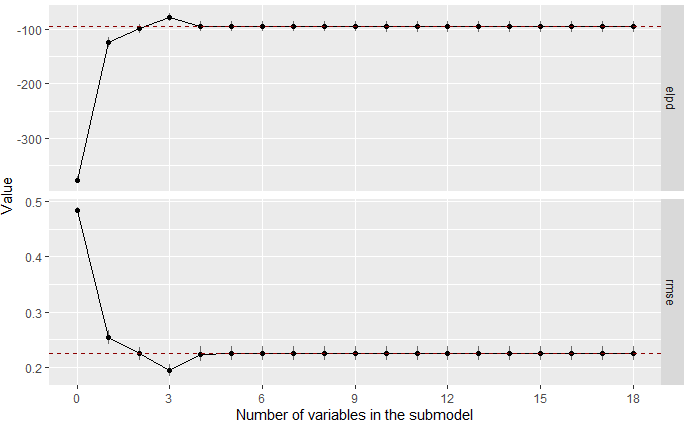
\includegraphics[width=0.8\linewidth]{images/cv_varsel} 

}

\caption{cv varsel function output}\label{fig:unnamed-chunk-18}
\end{figure}

The other reasoning behind the full model was which of the variables are
the best for obtaining better predictive performance. We can obtain a
ranking of best variables to be inserted in the model with
\texttt{solution\_terms}, and from this ranking we choose the first 3
best variables: \texttt{area\_worst}, \texttt{smoothness\_mean} and
\texttt{texture\_mean}.

\begin{figure}[H]

{\centering 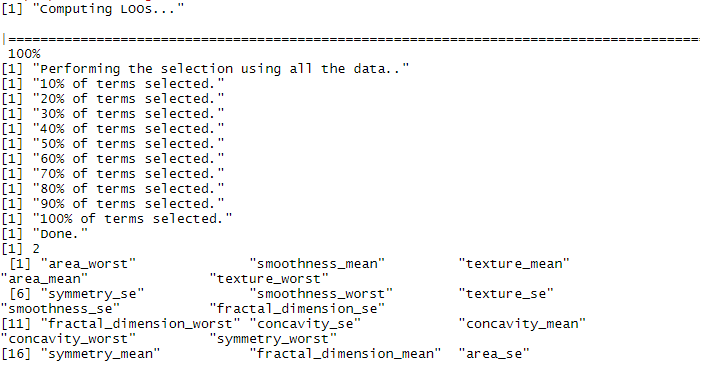
\includegraphics[width=0.8\linewidth]{images/solution_terms} 

}

\caption{solution terms function output}\label{fig:unnamed-chunk-19}
\end{figure}

Note: these functions are computationally complex and require quite a
large amount of time to be executed and we needed to run the code many
times to fix errors and other reasons. Because of this, the code block
has been made to pass the execution, but photos of the correct execution
have been inserted.

\hypertarget{multivariate-model---three-variables-model}{%
\subsection{Multivariate Model - Three Variables
Model}\label{multivariate-model---three-variables-model}}

This model is the result of applying projection predictive variable
selection to the full multivariate model of 18 variables. In this model
we simply take the 3 best variables obtained using the previous analysis
and study the outcomes.

\hypertarget{sampling-and-stan-code-1}{%
\subsubsection{Sampling and Stan Code}\label{sampling-and-stan-code-1}}

For this model, we used \texttt{generalized\ linear\ model},
\texttt{stan\_glm}, using the same prior distributions for the intercept
and regression coefficients as the previous models, this is:
\(\alpha \sim N(0,1)\) for the intercept coefficient and
\(\beta_n \sim StudentT(3,0,1)\) for the regression coefficient.

In order for the model to compute the predictions of the diagnosis
outcome we used binomial logistic regression, by making use of
\texttt{stan\_glm}'s \texttt{family} for which we chose
\texttt{binomial} with \texttt{link\ =\ "logit"}. The \texttt{.stan}
code can be found in the \protect\hyperlink{apb}{Appendix D - Model
Code} in the
\texttt{Multivariate\ Three\ Variables\ Model\ Stan\_GLM\ Code}.

The formula includes the 3 best ranked predictive variables and the
target.

\begin{Shaded}
\begin{Highlighting}[]
\NormalTok{multivariate_three <-}\StringTok{ }\KeywordTok{stan_glm}\NormalTok{(diagnosis }\OperatorTok{~}\StringTok{ }\NormalTok{area_worst }\OperatorTok{+}\StringTok{ }\NormalTok{smoothness_mean}
                               \OperatorTok{+}\StringTok{ }\NormalTok{texture_mean, }\DataTypeTok{data =}\NormalTok{ scaled_cancer_data,}
                               \DataTypeTok{family =} \KeywordTok{binomial}\NormalTok{(}\DataTypeTok{link =} \StringTok{"logit"}\NormalTok{), }
                               \DataTypeTok{prior =}\NormalTok{ beta, }\DataTypeTok{prior_intercept =}\NormalTok{ alpha,}
                               \DataTypeTok{seed =}\NormalTok{ SEED, }\DataTypeTok{refresh=}\DecValTok{0}\NormalTok{)}
\NormalTok{multivariate_glms <-}\StringTok{ }\KeywordTok{append}\NormalTok{(multivariate_glms, }\KeywordTok{list}\NormalTok{(multivariate_three))}
\end{Highlighting}
\end{Shaded}

\hypertarget{multivariate-model---regularized-horseshoe-model}{%
\subsection{Multivariate Model - Regularized Horseshoe
Model}\label{multivariate-model---regularized-horseshoe-model}}

As we already know that most of the variables are irrelevant thanks to
the previous projection predictive variable selection analysis, and only
three variables are relevant in order to obtain a better performance, we
decided to implement a Regularized Horseshoe Prior approach which has
been proven to be a worthy alternative.

\hypertarget{sampling-and-stan-code-2}{%
\subsubsection{Sampling and Stan Code}\label{sampling-and-stan-code-2}}

For this model, we used \texttt{generalized\ linear\ model},
\texttt{stan\_glm}, but instead of using the same priors for the
intercept and regression coefficients we use the weakly informative
regularized horseshoe prior which includes prior assumption that some of
the variables might be irrelevant.

This is the reason why we choose \(p_0 = 3\), and we pass this to the
regularized horseshoe prior, which will in turn use it to calculate the
respective distributions.

In order for the model to compute the predictions of the diagnosis
outcome we used binomial logistic regression, by making use of
\texttt{stan\_glm}'s \texttt{family} for which we chose
\texttt{binomial} with \texttt{link\ =\ "logit"}. The \texttt{.stan}
code can be found in the \protect\hyperlink{apb}{Appendix D - Model
Code} in the \texttt{Multivariate\ RHS\ Model\ Stan\_GLM\ Code}.

The formula for the regularized horseshoe prior is the same as the
multivariate model with all variables, it includes all of the 18
predictive variables and the target.

\begin{Shaded}
\begin{Highlighting}[]
\NormalTok{multivariate_rhsp <-}\StringTok{ }\KeywordTok{stan_glm}\NormalTok{(diagnosis }\OperatorTok{~}\StringTok{ }\NormalTok{texture_mean }\OperatorTok{+}\StringTok{ }\NormalTok{area_mean}
                              \OperatorTok{+}\StringTok{ }\NormalTok{smoothness_mean }\OperatorTok{+}\StringTok{ }\NormalTok{concavity_mean}
                              \OperatorTok{+}\StringTok{ }\NormalTok{symmetry_mean }\OperatorTok{+}\StringTok{ }\NormalTok{fractal_dimension_mean}
                              \OperatorTok{+}\StringTok{ }\NormalTok{texture_se }\OperatorTok{+}\StringTok{ }\NormalTok{area_se }\OperatorTok{+}\StringTok{ }\NormalTok{smoothness_se}
                              \OperatorTok{+}\StringTok{ }\NormalTok{concavity_se }\OperatorTok{+}\StringTok{ }\NormalTok{symmetry_se}
                              \OperatorTok{+}\StringTok{ }\NormalTok{fractal_dimension_se }\OperatorTok{+}\StringTok{ }\NormalTok{texture_worst}
                              \OperatorTok{+}\StringTok{ }\NormalTok{area_worst }\OperatorTok{+}\StringTok{ }\NormalTok{smoothness_worst }\OperatorTok{+}\StringTok{ }\NormalTok{concavity_worst}
                              \OperatorTok{+}\StringTok{ }\NormalTok{symmetry_worst }\OperatorTok{+}\StringTok{ }\NormalTok{fractal_dimension_worst,}
                              \DataTypeTok{data =}\NormalTok{ scaled_cancer_data,}
                              \DataTypeTok{family =} \KeywordTok{binomial}\NormalTok{(}\DataTypeTok{link =} \StringTok{"logit"}\NormalTok{),}
                              \DataTypeTok{prior=}\NormalTok{rhs_prior, }\DataTypeTok{QR=}\OtherTok{TRUE}\NormalTok{,}
                              \DataTypeTok{seed =}\NormalTok{ SEED, }\DataTypeTok{refresh=}\DecValTok{0}\NormalTok{)}
\NormalTok{multivariate_glms <-}\StringTok{ }\KeywordTok{append}\NormalTok{(multivariate_glms, }\KeywordTok{list}\NormalTok{(multivariate_rhsp))}
\end{Highlighting}
\end{Shaded}

\hypertarget{gaussian-model-1}{%
\subsection{Gaussian Model}\label{gaussian-model-1}}

The last model that was considered for this project was a Gaussian
Process based model. Gaussian models provide a probability distribution
over functions. They are useful for representing those datasets that
cannot be easily adjusted to a line following a regression procedure. A
gaussian process consists of generating higher degree polynomial
functions and assigning to those functions a probability. Therefore, by
taking the mean over the probability distribution, the most probable fit
is obtained.

\hypertarget{stan-code-2}{%
\subsubsection{Stan code}\label{stan-code-2}}

The common \textbf{stan code} for each variable is designed as follows:

\begin{Shaded}
\begin{Highlighting}[]
\KeywordTok{writeLines}\NormalTok{(}\KeywordTok{readLines}\NormalTok{(}\StringTok{"models/gaussian_process_bernoulli.stan"}\NormalTok{))}
\end{Highlighting}
\end{Shaded}

\begin{verbatim}
## data {
##   int<lower=1> N_obs;
##   real x_obs[N_obs];
##   int<lower=0, upper=1> y_obs[N_obs];
##   int<lower=1> N_predict;
##   real x_predict[N_predict];
## }
## transformed data {
##   real delta = 1e-9;
##   int<lower=1> N = N_obs + N_predict;
##   real x[N];
##   for (n_obs in 1:N_obs) x[n_obs] = x_obs[n_obs];
##   for (n_predict in 1:N_predict) x[N_obs + n_predict] = x_predict[n_predict];
## }
## parameters {
##   real<lower=0> rho;
##   real<lower=0> alpha;
##   real a;
##   vector[N] eta;
## }
## transformed parameters {
##   vector[N] f;
##   {
##     matrix[N, N] L_K;
##     matrix[N, N] K = cov_exp_quad(x, alpha, rho);
## 
##     // diagonal elements
##     for (n in 1:N)
##       K[n, n] = K[n, n] + delta;
## 
##     L_K = cholesky_decompose(K);
##     f = L_K * eta;
##   }
## }
## model {
##   rho ~ inv_gamma(1, 1);
##   alpha ~ std_normal();
##   a ~ std_normal();
##   eta ~ std_normal();
## 
##   y_obs ~ bernoulli_logit(a + f[1:N_obs]);
## }
## generated quantities {
##   int y_predict[N_predict];
##   vector[N_predict] log_lik;
##   for (n_predict in 1:N_predict){
##     y_predict[n_predict] = bernoulli_logit_rng(a + f[N_obs + n_predict]);
##     log_lik[n_predict] = bernoulli_logit_lpmf(y_obs[n_predict] | a + f[N_obs + n_predict]);
##   }
## }
\end{verbatim}

In order to later assess the performance of the gaussian model based on
the quality of its predictions, the data set is divided into two
subsets, one for ``training'' the model, containing a higher number of
observations, and another one for ``testing'' the model.

\begin{Shaded}
\begin{Highlighting}[]
\NormalTok{train_index <-}\StringTok{ }\KeywordTok{sample}\NormalTok{(}\DecValTok{1}\OperatorTok{:}\KeywordTok{nrow}\NormalTok{(scaled_cancer_data), }\FloatTok{0.8}\OperatorTok{*}\KeywordTok{nrow}\NormalTok{(scaled_cancer_data))}
\NormalTok{test_index <-}\StringTok{ }\KeywordTok{setdiff}\NormalTok{(}\DecValTok{1}\OperatorTok{:}\KeywordTok{nrow}\NormalTok{(scaled_cancer_data), train_index)}

\NormalTok{train_set <-scaled_cancer_data[train_index, ]}
\NormalTok{test_set <-}\StringTok{ }\NormalTok{scaled_cancer_data[test_index, ]}
\end{Highlighting}
\end{Shaded}

The gaussian model was carried out over the three best variables
contained in the set of optimal variables obtained using the previous
models.

\begin{Shaded}
\begin{Highlighting}[]
\NormalTok{variables_gaussian <-}\StringTok{ }\KeywordTok{c}\NormalTok{(}\StringTok{"area_worst"}\NormalTok{, }\StringTok{"smoothness_mean"}\NormalTok{, }\StringTok{"texture_mean"}\NormalTok{)}
\NormalTok{gaussian_fits <-}\StringTok{ }\KeywordTok{c}\NormalTok{()}
\NormalTok{x_predicts_idx <-}\StringTok{ }\KeywordTok{c}\NormalTok{()}
\NormalTok{N_obs <-}\StringTok{ }\DecValTok{200}
\NormalTok{N_predict <-}\StringTok{ }\DecValTok{100}
\NormalTok{gaussian_model <-}\StringTok{ }\NormalTok{rstan}\OperatorTok{::}\KeywordTok{stan_model}\NormalTok{(}\DataTypeTok{file =} 
                                      \StringTok{"models/gaussian_process_bernoulli.stan"}\NormalTok{)}
\end{Highlighting}
\end{Shaded}

From the training set, 200 randomly selected observations are
considered. Gaussian models are computationally slow, hence, using the
total number of observations would take much time. From the test set,
100 observations are chosen, also randomly.

\begin{Shaded}
\begin{Highlighting}[]
\ControlFlowTok{for}\NormalTok{ (variable }\ControlFlowTok{in}\NormalTok{ variables_gaussian)\{}
  \KeywordTok{cat}\NormalTok{(}\StringTok{"}\CharTok{\textbackslash{}n}\StringTok{Sampling from model with variable: "}\NormalTok{, variable, }\StringTok{"}\CharTok{\textbackslash{}n}\StringTok{"}\NormalTok{)}
\NormalTok{  x_obs_idx <-}\StringTok{ }\KeywordTok{sort}\NormalTok{(}\KeywordTok{sample}\NormalTok{(}\DecValTok{1}\OperatorTok{:}\KeywordTok{length}\NormalTok{(train_set[,variable]), N_obs))}
\NormalTok{  x_predict_idx <-}\StringTok{ }\KeywordTok{sort}\NormalTok{(}\KeywordTok{sample}\NormalTok{(}\DecValTok{1}\OperatorTok{:}\KeywordTok{length}\NormalTok{(test_set[,variable]), N_predict))}
\NormalTok{  x_predicts_idx <-}\StringTok{ }\KeywordTok{c}\NormalTok{(x_predicts_idx, x_predict_idx)}
\NormalTok{  gaussian_model_data <-}\StringTok{ }\KeywordTok{list}\NormalTok{(}\DataTypeTok{N_predict =}\NormalTok{ N_predict,}
                              \DataTypeTok{x_predict =}\NormalTok{ test_set[,variable][x_predict_idx],}
                              \DataTypeTok{N_obs =}\NormalTok{ N_obs,}
                              \DataTypeTok{x_obs =}\NormalTok{ train_set[,variable][x_obs_idx],}
                              \DataTypeTok{y_obs =}\NormalTok{ train_set[,}\StringTok{"diagnosis"}\NormalTok{][x_obs_idx])}
  
\NormalTok{  gaussian_fit <-rstan}\OperatorTok{::}\KeywordTok{sampling}\NormalTok{(gaussian_model, }\DataTypeTok{data =}\NormalTok{ gaussian_model_data,}
                                 \DataTypeTok{iter=}\DecValTok{1000}\NormalTok{, }\DataTypeTok{chains=}\DecValTok{2}\NormalTok{, }\DataTypeTok{refresh=}\DecValTok{0}\NormalTok{)}
\NormalTok{  gaussian_fits <-}\StringTok{ }\KeywordTok{c}\NormalTok{(gaussian_fits, gaussian_fit)}
\NormalTok{\}}
\end{Highlighting}
\end{Shaded}

\hypertarget{convergence-diagnostics}{%
\section{Convergence Diagnostics}\label{convergence-diagnostics}}

\hypertarget{diagnostic-metrics}{%
\subsection{Diagnostic Metrics}\label{diagnostic-metrics}}

The aim of this section is to assess the convergence of our models using
a variety of diagnostics:

\(\mathbf{\hat{R}}\) is a quantitative measure of convergence that will
be used to monitor if a group of chains has converged to the target
distribution. This can be done by comparing the between and within-chain
estimate for model parameters. If chains have not converged, meaning
that they have not mixed well, \(\hat{R}\) will be greater than one. If
chains have converged, the \(\hat{R}\) value will be virtually one.

\(\mathbf{Effective Sample Size (S_{eff})}\) is a quantitative measure
of efficiency that will be used to check when the weights are
problematic, as we could have vastly imbalanced weights. It represents
the number of independent samples required to obtain an importance
sampling estimate with about the same efficiency as if we would have
used all the samples. The \texttt{monitor} function gives us two crude
measures of effective sample size called Bulk\_ESS and Tail\_ESS (an
\(ESS > 100\) per chain is considered good).

\(\mathbf{Divergence}\) checking will be used to check if a divergence
arises when the simulated Hamiltonian trajectory departs from the true
trajectory as measured by departure of the Hamiltonian value from its
initial value. To evaluate this, we will use the function
\texttt{check\_hmc\_diagnostics}.

\hypertarget{linear-model-diagnostics}{%
\subsection{Linear Model Diagnostics}\label{linear-model-diagnostics}}

The diagnostics for the linear models can be seen in the
\protect\hyperlink{apa}{Appendix A - Linear models} \texttt{Monitor} and
\texttt{Divergences} outputs.

All \(\hat{R}\) values in the linear models were 1 or close to 1, which
means that the chains have converged.

Additionally, the ESS values are way higher than 100, which establishes
that our values are good.

Finally, we have obtained 0 divergences for all of our linear models.

\hypertarget{multivariate-model-diagnostics}{%
\subsection{Multivariate Model
Diagnostics}\label{multivariate-model-diagnostics}}

The diagnostics for the multivariate models can be seen in the
\protect\hyperlink{apb}{Appendix B - Multivariate models}
\texttt{Monitor} and \texttt{Divergences} outputs.

All \(\hat{R}\) values in the multivariate models were 1 or close to 1,
which means that the chains have converged.

Additionally, the ESS values are way higher than 100, which establishes
that our values are good.

All multivariate models turned great regarding divergences. It must be
noted that the full multivariate model was problematic regarding this
issue. At first, the model contained more than 300 divergences. To solve
this, we tried different values of adapt\_delta (0.95, 0.999) and
increased the number of iterations up to 5000. We also tried increasing
the number of chains but this wasn't a viable option as the
computational time increased to an unrealistic point. Although the
performance has improved considerably, some divergences still exist,
which may be caused by the model's chains not visiting parts of the
variable space with significant posterior mass leading to biased
estimates. It must be noted that the number of divergences should be
negligible as the full multivariate model only has 11 divergences out of
10000 iterations (0.11\%).

\hypertarget{gaussian-model-diagnostics}{%
\subsection{Gaussian Model
Diagnostics}\label{gaussian-model-diagnostics}}

In order to visually assess the convergence of the gaussian model, the
chains for the scalar parameters are plotted.
\includegraphics{report_files/figure-latex/unnamed-chunk-28-1.pdf}
\includegraphics{report_files/figure-latex/unnamed-chunk-28-2.pdf}
\includegraphics{report_files/figure-latex/unnamed-chunk-28-3.pdf}

As in previous cases, the values obtained from applying the function
\texttt{monitor}are satisfactory. \(\hat{R}\) provides a valid scalar
metric for convergence checking based on computing the division between
the pooled variance of the chains and the individual variance of each of
them. Obtaining values close to 1, as in the current case, means that
the chains happen to have very similar distributions. Finally, the
results yielded for the effective sample size are higher than 100.

\hypertarget{posterior-predictive-checking}{%
\section{Posterior Predictive
Checking}\label{posterior-predictive-checking}}

\hypertarget{linear-models-1}{%
\subsection{Linear Models}\label{linear-models-1}}

Kernel density estimate for the data and posterior predictive replicates
of the linear models are slightly similar. From this we noticed that
some variables might be worst for predictions, such as all of the
\texttt{se} variables (`\texttt{texture\_se}, \texttt{symmetry\_se},
etc.).

\begin{Shaded}
\begin{Highlighting}[]
\NormalTok{y_sims <-}\StringTok{ }\KeywordTok{list}\NormalTok{()}
\ControlFlowTok{for}\NormalTok{ (model }\ControlFlowTok{in}\NormalTok{ linear_models)\{}
\NormalTok{  params <-}\StringTok{ }\KeywordTok{extract}\NormalTok{(model)}
\NormalTok{  y_sims <-}\StringTok{ }\KeywordTok{append}\NormalTok{(y_sims, }\KeywordTok{list}\NormalTok{(params}\OperatorTok{$}\NormalTok{y_sim[}\DecValTok{1}\OperatorTok{:}\DecValTok{100}\NormalTok{,]))}
\NormalTok{\}}

\NormalTok{ppc1 <-}\StringTok{ }\KeywordTok{ppc_dens_overlay}\NormalTok{(scaled_cancer_data}\OperatorTok{$}\NormalTok{diagnosis, y_sims[[}\DecValTok{1}\NormalTok{]])}
\NormalTok{ppc2 <-}\StringTok{ }\KeywordTok{ppc_dens_overlay}\NormalTok{(scaled_cancer_data}\OperatorTok{$}\NormalTok{diagnosis, y_sims[[}\DecValTok{2}\NormalTok{]])}
\NormalTok{ppc3 <-}\StringTok{ }\KeywordTok{ppc_dens_overlay}\NormalTok{(scaled_cancer_data}\OperatorTok{$}\NormalTok{diagnosis, y_sims[[}\DecValTok{3}\NormalTok{]])}
\NormalTok{ppc4 <-}\StringTok{ }\KeywordTok{ppc_dens_overlay}\NormalTok{(scaled_cancer_data}\OperatorTok{$}\NormalTok{diagnosis, y_sims[[}\DecValTok{4}\NormalTok{]])}
\NormalTok{ppc5 <-}\StringTok{ }\KeywordTok{ppc_dens_overlay}\NormalTok{(scaled_cancer_data}\OperatorTok{$}\NormalTok{diagnosis, y_sims[[}\DecValTok{5}\NormalTok{]])}
\NormalTok{ppc6 <-}\StringTok{ }\KeywordTok{ppc_dens_overlay}\NormalTok{(scaled_cancer_data}\OperatorTok{$}\NormalTok{diagnosis, y_sims[[}\DecValTok{6}\NormalTok{]])}
\NormalTok{ppc7 <-}\StringTok{ }\KeywordTok{ppc_dens_overlay}\NormalTok{(scaled_cancer_data}\OperatorTok{$}\NormalTok{diagnosis, y_sims[[}\DecValTok{7}\NormalTok{]])}
\NormalTok{ppc8 <-}\StringTok{ }\KeywordTok{ppc_dens_overlay}\NormalTok{(scaled_cancer_data}\OperatorTok{$}\NormalTok{diagnosis, y_sims[[}\DecValTok{8}\NormalTok{]])}
\NormalTok{ppc9 <-}\StringTok{ }\KeywordTok{ppc_dens_overlay}\NormalTok{(scaled_cancer_data}\OperatorTok{$}\NormalTok{diagnosis, y_sims[[}\DecValTok{9}\NormalTok{]])}
\NormalTok{ppc10 <-}\StringTok{ }\KeywordTok{ppc_dens_overlay}\NormalTok{(scaled_cancer_data}\OperatorTok{$}\NormalTok{diagnosis, y_sims[[}\DecValTok{10}\NormalTok{]])}
\NormalTok{ppc11 <-}\StringTok{ }\KeywordTok{ppc_dens_overlay}\NormalTok{(scaled_cancer_data}\OperatorTok{$}\NormalTok{diagnosis, y_sims[[}\DecValTok{11}\NormalTok{]])}
\NormalTok{ppc12 <-}\StringTok{ }\KeywordTok{ppc_dens_overlay}\NormalTok{(scaled_cancer_data}\OperatorTok{$}\NormalTok{diagnosis, y_sims[[}\DecValTok{12}\NormalTok{]])}
\NormalTok{ppc13 <-}\StringTok{ }\KeywordTok{ppc_dens_overlay}\NormalTok{(scaled_cancer_data}\OperatorTok{$}\NormalTok{diagnosis, y_sims[[}\DecValTok{13}\NormalTok{]])}
\NormalTok{ppc14 <-}\StringTok{ }\KeywordTok{ppc_dens_overlay}\NormalTok{(scaled_cancer_data}\OperatorTok{$}\NormalTok{diagnosis, y_sims[[}\DecValTok{14}\NormalTok{]])}
\NormalTok{ppc15 <-}\StringTok{ }\KeywordTok{ppc_dens_overlay}\NormalTok{(scaled_cancer_data}\OperatorTok{$}\NormalTok{diagnosis, y_sims[[}\DecValTok{15}\NormalTok{]])}
\NormalTok{ppc16 <-}\StringTok{ }\KeywordTok{ppc_dens_overlay}\NormalTok{(scaled_cancer_data}\OperatorTok{$}\NormalTok{diagnosis, y_sims[[}\DecValTok{16}\NormalTok{]])}
\NormalTok{ppc17 <-}\StringTok{ }\KeywordTok{ppc_dens_overlay}\NormalTok{(scaled_cancer_data}\OperatorTok{$}\NormalTok{diagnosis, y_sims[[}\DecValTok{17}\NormalTok{]])}
\NormalTok{ppc18 <-}\StringTok{ }\KeywordTok{ppc_dens_overlay}\NormalTok{(scaled_cancer_data}\OperatorTok{$}\NormalTok{diagnosis, y_sims[[}\DecValTok{18}\NormalTok{]])}

\KeywordTok{bayesplot_grid}\NormalTok{(ppc1, ppc2, ppc3, ppc4, ppc5, ppc6,}
               \DataTypeTok{subtitles =} \KeywordTok{c}\NormalTok{(}\StringTok{"texture_mean"}\NormalTok{, }\StringTok{"area_mean"}\NormalTok{,}
                             \StringTok{"smoothness_mean"}\NormalTok{, }\StringTok{"concavity_mean"}\NormalTok{,}
                             \StringTok{"symmetry_mean"}\NormalTok{, }\StringTok{"fractal_dimension_mean"}\NormalTok{))}
\end{Highlighting}
\end{Shaded}

\includegraphics{report_files/figure-latex/unnamed-chunk-29-1.pdf}

\begin{Shaded}
\begin{Highlighting}[]
\KeywordTok{bayesplot_grid}\NormalTok{(ppc7, ppc8, ppc9, ppc10, ppc11, ppc12,}
               \DataTypeTok{subtitles =} \KeywordTok{c}\NormalTok{(}\StringTok{"texture_se"}\NormalTok{, }\StringTok{"area_se"}\NormalTok{,}
                             \StringTok{"smoothness_se"}\NormalTok{, }\StringTok{"concavity_se"}\NormalTok{,}
                             \StringTok{"symmetry_se"}\NormalTok{, }\StringTok{"fractal_dimension_se"}\NormalTok{))}
\end{Highlighting}
\end{Shaded}

\includegraphics{report_files/figure-latex/unnamed-chunk-29-2.pdf}

\begin{Shaded}
\begin{Highlighting}[]
\KeywordTok{bayesplot_grid}\NormalTok{(ppc13, ppc14, ppc15, ppc16, ppc17, ppc18,}
               \DataTypeTok{subtitles =} \KeywordTok{c}\NormalTok{(}\StringTok{"texture_worst"}\NormalTok{, }\StringTok{"area_worst"}\NormalTok{,}
                             \StringTok{"smoothness_worst"}\NormalTok{, }\StringTok{"concavity_worst"}\NormalTok{, }
                             \StringTok{"symmetry_worst"}\NormalTok{, }\StringTok{"fractal_dimension_worst"}\NormalTok{))}
\end{Highlighting}
\end{Shaded}

\includegraphics{report_files/figure-latex/unnamed-chunk-29-3.pdf}

\hypertarget{multivariate-models}{%
\subsection{Multivariate Models}\label{multivariate-models}}

In the posterior predictive checking for each of the variable blocks, it
is noticeable how much less the \texttt{se} block can influence the
fitting of the model and thus getting better predictive results with
these variables might not be a viable option. This is corroborated by
the linear model predictive checking.

The \texttt{full}, \texttt{three\ variables} and \texttt{rhs}
multivariate models have relatively similar kernel density estimate for
the data.

\begin{Shaded}
\begin{Highlighting}[]
\NormalTok{y_sims <-}\StringTok{ }\KeywordTok{list}\NormalTok{()}
\ControlFlowTok{for}\NormalTok{ (model }\ControlFlowTok{in}\NormalTok{ multivariate_glms)\{}
\NormalTok{  params <-}\StringTok{ }\KeywordTok{posterior_predict}\NormalTok{(model, }\DataTypeTok{draws =} \DecValTok{100}\NormalTok{)}
  \KeywordTok{head}\NormalTok{(params)}
\NormalTok{  y_sims <-}\StringTok{ }\KeywordTok{append}\NormalTok{(y_sims, }\KeywordTok{list}\NormalTok{(params))}
\NormalTok{\}}

\NormalTok{ppc_mv_}\DecValTok{1}\NormalTok{ <-}\StringTok{ }\KeywordTok{ppc_dens_overlay}\NormalTok{(scaled_cancer_data}\OperatorTok{$}\NormalTok{diagnosis, y_sims[[}\DecValTok{1}\NormalTok{]])}
\NormalTok{ppc_mv_}\DecValTok{2}\NormalTok{ <-}\StringTok{ }\KeywordTok{ppc_dens_overlay}\NormalTok{(scaled_cancer_data}\OperatorTok{$}\NormalTok{diagnosis, y_sims[[}\DecValTok{2}\NormalTok{]])}
\NormalTok{ppc_mv_}\DecValTok{3}\NormalTok{ <-}\StringTok{ }\KeywordTok{ppc_dens_overlay}\NormalTok{(scaled_cancer_data}\OperatorTok{$}\NormalTok{diagnosis, y_sims[[}\DecValTok{3}\NormalTok{]])}
\NormalTok{ppc_mv_}\DecValTok{4}\NormalTok{ <-}\StringTok{ }\KeywordTok{ppc_dens_overlay}\NormalTok{(scaled_cancer_data}\OperatorTok{$}\NormalTok{diagnosis, y_sims[[}\DecValTok{4}\NormalTok{]])}
\NormalTok{ppc_mv_}\DecValTok{5}\NormalTok{ <-}\StringTok{ }\KeywordTok{ppc_dens_overlay}\NormalTok{(scaled_cancer_data}\OperatorTok{$}\NormalTok{diagnosis, y_sims[[}\DecValTok{5}\NormalTok{]])}
\NormalTok{ppc_mv_}\DecValTok{6}\NormalTok{ <-}\StringTok{ }\KeywordTok{ppc_dens_overlay}\NormalTok{(scaled_cancer_data}\OperatorTok{$}\NormalTok{diagnosis, y_sims[[}\DecValTok{6}\NormalTok{]])}

\KeywordTok{bayesplot_grid}\NormalTok{(ppc_mv_}\DecValTok{1}\NormalTok{, ppc_mv_}\DecValTok{2}\NormalTok{, ppc_mv_}\DecValTok{3}\NormalTok{, ppc_mv_}\DecValTok{4}\NormalTok{, ppc_mv_}\DecValTok{5}\NormalTok{, ppc_mv_}\DecValTok{6}\NormalTok{,}
               \DataTypeTok{subtitles =} \KeywordTok{c}\NormalTok{(}\StringTok{"Mean Model"}\NormalTok{, }\StringTok{"SE Model"}\NormalTok{,}
                             \StringTok{"Worst Model"}\NormalTok{, }\StringTok{"Full Model"}\NormalTok{,}
                             \StringTok{"Three Variables Model"}\NormalTok{, }\StringTok{"RHS Model"}\NormalTok{))}
\end{Highlighting}
\end{Shaded}

\includegraphics{report_files/figure-latex/unnamed-chunk-30-1.pdf}

\hypertarget{gaussian-model-2}{%
\subsection{Gaussian Model}\label{gaussian-model-2}}

The density of the diagnosis in the test set is printed in black color.
Overlapping, the densities for the predictions of the first 50
iterations. This graph enables visual assessment of the quality of the
predictions. Preliminarly, the results seem to be satisfactory.

\includegraphics{report_files/figure-latex/unnamed-chunk-31-1.pdf}
\includegraphics{report_files/figure-latex/unnamed-chunk-31-2.pdf}
\includegraphics{report_files/figure-latex/unnamed-chunk-31-3.pdf}

Another way to check if the predicted samples represent the reality is
by directly plotting them (orange) and comparing with the target ones
(grey). This is possible because the gaussian model is applied on values
that are contained in the test set for the chosen variable. The
concentration of points at 0 or 1 \emph{y} values should be similar for
the same values of \emph{x}. In the given cases, by looking at the
graphs, there is a very similar tendency between the real values and the
simulated ones, meaning that the result is good.

\includegraphics{report_files/figure-latex/unnamed-chunk-32-1.pdf}
\includegraphics{report_files/figure-latex/unnamed-chunk-32-2.pdf}
\includegraphics{report_files/figure-latex/unnamed-chunk-32-3.pdf}

\hypertarget{model-comparisons}{%
\section{Model comparisons}\label{model-comparisons}}

For model comparison we compare the models with \textbf{Leave-One-Out
Cross Validation} (PSIS-LOO) and we assess the \(\hat{k}\)-values
reliability for each of the models. If for the latter for the
\(\hat{k}\)-values of a model are equal or lower than 0.7 we can
consider that the model is reliable.

\hypertarget{linear-models-2}{%
\subsection{Linear Models}\label{linear-models-2}}

We obtain the PSIS-LOO estimates for each of the linear models as well
as their respective \(\hat{k}\)-values.

By looking at the \texttt{elpd\_loo} and \texttt{p\_loo} values for each
of the models, we can deduce that the most reliable variables to be used
are as follows (in order of best): \texttt{area\_worst},
\texttt{area\_mean}, \texttt{area\_se}, \texttt{concavity\_mean}.

\begin{table}[H]
\centering
\begin{tabular}{|l|l|l|}
\hline
\textbf{Variable}   & \textbf{elpd\_loo} & \textbf{p\_loo} \\ \hline
14 - area\_worst    & -117.29            & 1.89            \\ \hline
2 - area\_mean      & -164.88            & 2.00            \\ \hline
8 - area\_se        & -181.79            & 2.20            \\ \hline
4 - concavity\_mean & -194.48            & 3.58            \\ \hline
\end{tabular}
\caption{Most reliable linear models.}
\end{table}

\begin{Shaded}
\begin{Highlighting}[]
\NormalTok{pareto_k_values <-}\StringTok{ }\KeywordTok{list}\NormalTok{()}
\NormalTok{linear_loo_estimates_df <-}\StringTok{ }\KeywordTok{data.frame}\NormalTok{()}

\ControlFlowTok{for}\NormalTok{ (i }\ControlFlowTok{in}\NormalTok{ (}\DecValTok{1}\OperatorTok{:}\KeywordTok{length}\NormalTok{(linear_models)))\{}
  \KeywordTok{cat}\NormalTok{(}\StringTok{"- Monitoring variable: "}\NormalTok{, variables[i], }\StringTok{"}\CharTok{\textbackslash{}n}\StringTok{"}\NormalTok{)}
\NormalTok{  model <-}\StringTok{ }\NormalTok{linear_models[[i]]}
\NormalTok{  model_log_lik <-}\StringTok{ }\KeywordTok{extract_log_lik}\NormalTok{(model, }\DataTypeTok{parameter_name =} \StringTok{"log_lik"}\NormalTok{,}
                                   \DataTypeTok{merge_chains =} \OtherTok{FALSE}\NormalTok{)}
\NormalTok{  model_r_eff <-}\StringTok{ }\KeywordTok{relative_eff}\NormalTok{(}\KeywordTok{exp}\NormalTok{(model_log_lik))}
\NormalTok{  model_loo <-}\StringTok{ }\KeywordTok{loo}\NormalTok{(model_log_lik, }\DataTypeTok{r_eff =}\NormalTok{ model_r_eff)}
\NormalTok{  pareto_k_values <-}\StringTok{ }\KeywordTok{append}\NormalTok{(pareto_k_values,}
                            \KeywordTok{list}\NormalTok{(model_loo}\OperatorTok{$}\NormalTok{diagnostics}\OperatorTok{$}\NormalTok{pareto_k))}
  
\NormalTok{  y_pred <-}\StringTok{ }\KeywordTok{as.vector}\NormalTok{(}\KeywordTok{extract}\NormalTok{(linear_models[[i]], }\DataTypeTok{pars=}\StringTok{"y_sim"}\NormalTok{))}
\NormalTok{  preds <-}\StringTok{ }\KeywordTok{colMeans}\NormalTok{(y_pred}\OperatorTok{$}\NormalTok{y_sim)}
\NormalTok{  pr <-}\StringTok{ }\KeywordTok{as.integer}\NormalTok{(preds }\OperatorTok{>=}\StringTok{ }\FloatTok{0.5}\NormalTok{)}
\NormalTok{  acc <-}\StringTok{ }\KeywordTok{round}\NormalTok{(}\KeywordTok{mean}\NormalTok{(}\KeywordTok{xor}\NormalTok{(pr, }\KeywordTok{as.integer}\NormalTok{(scaled_cancer_data}\OperatorTok{$}\NormalTok{diagnosis}\OperatorTok{==}\DecValTok{0}\NormalTok{))), }\DecValTok{4}\NormalTok{)}

\NormalTok{  aux_df <-}\StringTok{ }\KeywordTok{data.frame}\NormalTok{(}\StringTok{"variable"}\NormalTok{ =}\StringTok{ }\NormalTok{variables[i],}
                       \StringTok{"elpd_loo"}\NormalTok{ =}\StringTok{ }\NormalTok{model_loo}\OperatorTok{$}\NormalTok{estimates[}\DecValTok{1}\NormalTok{],}
                       \StringTok{"p_loo"}\NormalTok{ =}\StringTok{ }\NormalTok{model_loo}\OperatorTok{$}\NormalTok{estimates[}\DecValTok{2}\NormalTok{],}
                       \StringTok{"accuracy"}\NormalTok{ =}\StringTok{ }\NormalTok{acc)}

\NormalTok{  linear_loo_estimates_df <-}\StringTok{ }\KeywordTok{rbind}\NormalTok{(linear_loo_estimates_df, aux_df)}
\NormalTok{\}}
\end{Highlighting}
\end{Shaded}

\begin{verbatim}
## - Monitoring variable:  texture_mean 
## - Monitoring variable:  area_mean
\end{verbatim}

\begin{verbatim}
## Warning: Some Pareto k diagnostic values are too high. See help('pareto-k-diagnostic') for details.
\end{verbatim}

\begin{verbatim}
## - Monitoring variable:  smoothness_mean 
## - Monitoring variable:  concavity_mean 
## - Monitoring variable:  symmetry_mean 
## - Monitoring variable:  fractal_dimension_mean 
## - Monitoring variable:  texture_se 
## - Monitoring variable:  area_se
\end{verbatim}

\begin{verbatim}
## Warning: Some Pareto k diagnostic values are too high. See help('pareto-k-diagnostic') for details.
\end{verbatim}

\begin{verbatim}
## - Monitoring variable:  smoothness_se 
## - Monitoring variable:  concavity_se
\end{verbatim}

\begin{verbatim}
## Warning: Some Pareto k diagnostic values are slightly high. See help('pareto-k-diagnostic') for details.
\end{verbatim}

\begin{verbatim}
## - Monitoring variable:  symmetry_se 
## - Monitoring variable:  fractal_dimension_se 
## - Monitoring variable:  texture_worst 
## - Monitoring variable:  area_worst
\end{verbatim}

\begin{verbatim}
## Warning: Some Pareto k diagnostic values are too high. See help('pareto-k-diagnostic') for details.
\end{verbatim}

\begin{verbatim}
## - Monitoring variable:  smoothness_worst 
## - Monitoring variable:  concavity_worst 
## - Monitoring variable:  symmetry_worst 
## - Monitoring variable:  fractal_dimension_worst
\end{verbatim}

\begin{Shaded}
\begin{Highlighting}[]
\KeywordTok{print}\NormalTok{(linear_loo_estimates_df)}
\end{Highlighting}
\end{Shaded}

\begin{verbatim}
##                   variable  elpd_loo    p_loo accuracy
## 1             texture_mean -325.3444 2.230660   0.6977
## 2                area_mean -164.8824 2.000459   0.8822
## 3          smoothness_mean -339.0114 2.107357   0.6678
## 4           concavity_mean -194.4851 3.579987   0.8822
## 5            symmetry_mean -345.4021 2.037845   0.6837
## 6   fractal_dimension_mean -377.6696 2.027334   0.6274
## 7               texture_se -377.7236 1.975586   0.6274
## 8                  area_se -181.7876 2.025407   0.8682
## 9            smoothness_se -376.4835 2.183166   0.6274
## 10            concavity_se -357.6228 5.913835   0.6555
## 11             symmetry_se -377.8206 2.220651   0.6274
## 12    fractal_dimension_se -376.3487 2.481702   0.6186
## 13           texture_worst -313.1982 2.233350   0.7223
## 14              area_worst -117.2949 1.886005   0.9104
## 15        smoothness_worst -322.7422 2.060363   0.7153
## 16         concavity_worst -221.6281 3.419314   0.8471
## 17          symmetry_worst -326.3961 1.568806   0.7118
## 18 fractal_dimension_worst -348.6119 1.795104   0.6907
\end{verbatim}

Most of the models have exceptional \(\hat{k}\)-values (lower than 0.7),
which means that the results obtained by the models are reliable. The
following output visualizes the Pareto-k values for each linear model.

\begin{Shaded}
\begin{Highlighting}[]
\NormalTok{p <-}\StringTok{ }\KeywordTok{list}\NormalTok{()}
\ControlFlowTok{for}\NormalTok{ (i }\ControlFlowTok{in} \DecValTok{1}\OperatorTok{:}\KeywordTok{length}\NormalTok{(pareto_k_values))\{}
\NormalTok{  df <-}\StringTok{ }\KeywordTok{data.frame}\NormalTok{(pareto_k_values[[i]])}
  \KeywordTok{colnames}\NormalTok{(df) <-}\StringTok{ }\KeywordTok{c}\NormalTok{(}\StringTok{"values"}\NormalTok{)}
\NormalTok{  p[[i]] <-}\StringTok{ }\KeywordTok{ggplot}\NormalTok{(}\DataTypeTok{data=}\NormalTok{df, }\KeywordTok{aes}\NormalTok{(}\DataTypeTok{y=}\NormalTok{values, }\DataTypeTok{x=}\DecValTok{1}\OperatorTok{:}\KeywordTok{nrow}\NormalTok{(cancer_data))) }\OperatorTok{+}
\StringTok{    }\KeywordTok{geom_point}\NormalTok{(}\DataTypeTok{color=}\StringTok{"#10A5F5"}\NormalTok{) }\OperatorTok{+}
\StringTok{    }\KeywordTok{geom_hline}\NormalTok{(}\DataTypeTok{yintercept=}\FloatTok{0.7}\NormalTok{, }\DataTypeTok{linetype=}\StringTok{"dashed"}\NormalTok{, }\DataTypeTok{size=}\DecValTok{1}\NormalTok{, }\DataTypeTok{color=}\StringTok{"#0859C6"}\NormalTok{) }\OperatorTok{+}
\StringTok{    }\KeywordTok{ggtitle}\NormalTok{(variables[i]) }\OperatorTok{+}\StringTok{  }\KeywordTok{xlab}\NormalTok{(}\StringTok{"Samples"}\NormalTok{) }\OperatorTok{+}\StringTok{ }\KeywordTok{ylab}\NormalTok{(}\StringTok{"K-values"}\NormalTok{)}
\NormalTok{\}}
\KeywordTok{do.call}\NormalTok{(grid.arrange, }\KeywordTok{c}\NormalTok{(p[}\DecValTok{1}\OperatorTok{:}\DecValTok{6}\NormalTok{], }\DataTypeTok{ncol=}\DecValTok{3}\NormalTok{))}
\end{Highlighting}
\end{Shaded}

\includegraphics{report_files/figure-latex/unnamed-chunk-34-1.pdf}

\begin{Shaded}
\begin{Highlighting}[]
\KeywordTok{do.call}\NormalTok{(grid.arrange, }\KeywordTok{c}\NormalTok{(p[}\DecValTok{7}\OperatorTok{:}\DecValTok{12}\NormalTok{], }\DataTypeTok{ncol=}\DecValTok{3}\NormalTok{))}
\end{Highlighting}
\end{Shaded}

\includegraphics{report_files/figure-latex/unnamed-chunk-34-2.pdf}

\begin{Shaded}
\begin{Highlighting}[]
\KeywordTok{do.call}\NormalTok{(grid.arrange, }\KeywordTok{c}\NormalTok{(p[}\DecValTok{13}\OperatorTok{:}\DecValTok{18}\NormalTok{], }\DataTypeTok{ncol=}\DecValTok{3}\NormalTok{))}
\end{Highlighting}
\end{Shaded}

\includegraphics{report_files/figure-latex/unnamed-chunk-34-3.pdf}

\hypertarget{multivariate-models-1}{%
\subsection{Multivariate Models}\label{multivariate-models-1}}

We obtain the PSIS-LOO estimates for each of the multivariate models as
well as their respective \(\hat{k}\)-values.

What we take out of the analysis by variable blocks is that, in general,
the \texttt{se} variables might not be as influential for predictions as
the other blocks. Although this analysis did not bring a more specific
result, it was an interesting experiment to carry out in order to check
if any of the variable blocks might influence the final model too badly.

For the other models: \texttt{Full\ Variables\ Model},
\texttt{Three\ Variables\ Model} and \texttt{RHS\ Model}, the results
are as we expected from before starting the analysis. The results for
the \texttt{Full\ Variables\ Model} show that it isn't viable to use all
of the 18 variables, because we obtain even better results by using the
optimal number of variables and the specific variables we obtained from
the projection predictive variable selection analysis, as can be seen in
the results of \texttt{Three\ Variables\ Model} and \texttt{RHS\ Model}.

\begin{table}[H]
\centering
\begin{tabular}{|l|l|l|}
\hline
\textbf{variable.group} & \textbf{elpd\_loo} & \textbf{p\_loo} \\ \hline
1 Mean Model            & -83.85             & 5.68            \\ \hline
2 SE Model              & -173.03            & 12.22           \\ \hline
3 Worst Model           & -57.17             & 2.76            \\ \hline
4 Full Variables Model  & -95.77             & 5.78            \\ \hline
5 Three variables Model & -63.92             & 3.34            \\ \hline
6 RHS Model             & -48.70             & 14.45           \\ \hline
\end{tabular}
\end{table}

\begin{Shaded}
\begin{Highlighting}[]
\CommentTok{# Auxiliary function to calculate the accuracy of a model}
\NormalTok{model_accuracies <-}\StringTok{ }\ControlFlowTok{function}\NormalTok{(model)\{}
\NormalTok{  y_pred <-}\StringTok{ }\KeywordTok{posterior_epred}\NormalTok{(model)}
\NormalTok{  preds <-}\StringTok{ }\KeywordTok{colMeans}\NormalTok{(y_pred)}
\NormalTok{  pr <-}\StringTok{ }\KeywordTok{as.integer}\NormalTok{(preds }\OperatorTok{>=}\StringTok{ }\FloatTok{0.5}\NormalTok{)}
\NormalTok{  acc <-}\StringTok{ }\KeywordTok{round}\NormalTok{(}\KeywordTok{mean}\NormalTok{(}\KeywordTok{xor}\NormalTok{(pr, }\KeywordTok{as.integer}\NormalTok{(scaled_cancer_data}\OperatorTok{$}\NormalTok{diagnosis}\OperatorTok{==}\DecValTok{0}\NormalTok{))), }\DecValTok{4}\NormalTok{)}
  
\NormalTok{  conf_matrix <-}\StringTok{ }\KeywordTok{confusionMatrix}\NormalTok{(}\KeywordTok{factor}\NormalTok{(}\KeywordTok{round}\NormalTok{(pr)), }
                                 \KeywordTok{factor}\NormalTok{(scaled_cancer_data}\OperatorTok{$}\NormalTok{diagnosis))}
  \KeywordTok{return}\NormalTok{ (}\KeywordTok{list}\NormalTok{(acc, }\KeywordTok{list}\NormalTok{(conf_matrix)))}
\NormalTok{\}}
\end{Highlighting}
\end{Shaded}

\begin{Shaded}
\begin{Highlighting}[]
\NormalTok{pareto_k_values <-}\StringTok{ }\KeywordTok{list}\NormalTok{()}
\NormalTok{multivariate_loo_estimates_df <-}\StringTok{ }\KeywordTok{data.frame}\NormalTok{()}

\ControlFlowTok{for}\NormalTok{ (i }\ControlFlowTok{in}\NormalTok{ (}\DecValTok{1}\OperatorTok{:}\KeywordTok{length}\NormalTok{(multivariate_glms)))\{}
\NormalTok{  model <-}\StringTok{ }\NormalTok{multivariate_glms[[i]]}
  
\NormalTok{  model_log_lik <-}\StringTok{ }\KeywordTok{log_lik}\NormalTok{(model)}
\NormalTok{  model_loo <-}\StringTok{ }\KeywordTok{loo}\NormalTok{(model_log_lik)}
\NormalTok{  pareto_k_values <-}\StringTok{ }\KeywordTok{append}\NormalTok{(pareto_k_values, }
                            \KeywordTok{list}\NormalTok{(model_loo}\OperatorTok{$}\NormalTok{diagnostics}\OperatorTok{$}\NormalTok{pareto_k))}
  \KeywordTok{cat}\NormalTok{(}\StringTok{"}\CharTok{\textbackslash{}n}\StringTok{-- Monitoring Model: "}\NormalTok{, mv_model_names[i], }\StringTok{"-- }\CharTok{\textbackslash{}n}\StringTok{"}\NormalTok{)}
  \CommentTok{#print(model_loo)}
  
\NormalTok{  accs <-}\StringTok{ }\KeywordTok{model_accuracies}\NormalTok{(}\DataTypeTok{model =}\NormalTok{ multivariate_glms[[i]])}
  
\NormalTok{  aux_df <-}\StringTok{ }\KeywordTok{data.frame}\NormalTok{(}\StringTok{"variable group"}\NormalTok{ =}\StringTok{ }\NormalTok{mv_model_names[i],}
                       \StringTok{"elpd_loo"}\NormalTok{ =}\StringTok{ }\NormalTok{model_loo}\OperatorTok{$}\NormalTok{estimates[}\DecValTok{1}\NormalTok{],}
                       \StringTok{"p_loo"}\NormalTok{ =}\StringTok{ }\NormalTok{model_loo}\OperatorTok{$}\NormalTok{estimates[}\DecValTok{2}\NormalTok{],}
                       \StringTok{"accuracy"}\NormalTok{ =}\StringTok{ }\NormalTok{accs[[}\DecValTok{1}\NormalTok{]])}
  
\NormalTok{  multivariate_loo_estimates_df <-}\StringTok{ }\KeywordTok{rbind}\NormalTok{(multivariate_loo_estimates_df, aux_df)}
\NormalTok{\}}
\end{Highlighting}
\end{Shaded}

\begin{verbatim}
## 
## -- Monitoring Model:  Mean Model -- 
## 
## -- Monitoring Model:  SE Model -- 
## 
## -- Monitoring Model:  Worst Model -- 
## 
## -- Monitoring Model:  Full Variables Model -- 
## 
## -- Monitoring Model:  Three variables Model -- 
## 
## -- Monitoring Model:  RHS Model --
\end{verbatim}

\begin{Shaded}
\begin{Highlighting}[]
\KeywordTok{print}\NormalTok{(multivariate_loo_estimates_df)}
\end{Highlighting}
\end{Shaded}

\begin{verbatim}
##          variable.group   elpd_loo     p_loo accuracy
## 1            Mean Model  -83.84899  5.676937   0.9438
## 2              SE Model -173.02859 12.218856   0.8910
## 3           Worst Model  -57.17492  2.763165   0.9719
## 4  Full Variables Model  -95.77037  5.779921   0.9332
## 5 Three variables Model  -63.91804  3.344444   0.9543
## 6             RHS Model  -48.70333 14.446112   0.9859
\end{verbatim}

All of the multivariate variable block models have relatively
exceptional \(\hat{k}\)-values (lower than 0.7), with a few high
exceptions (equal or higher than 0.7), which means that the results
obtained by the models are relatively reliable.

For the \texttt{Full\ Variables\ Model} and
\texttt{Three\ Variables\ Model}, we obtain relatively decent
\(\hat{k}\)-values, with a few more high exceptions than for the
variable block models. On the other hand, for the \texttt{RHS\ Model},
the \(\hat{k}\)-values are mediocre, as there is a high amount (14\%) of
higher than 0.7 values. Even though we obtain better PSIS-LOO and
predictive results than for the previous models, we must be aware of the
fact that \texttt{Full\ Variables\ Model},
\texttt{Three\ Variables\ Model} and \texttt{RHS\ Model} \textbf{may} be
considered unreliable.

\begin{Shaded}
\begin{Highlighting}[]
\NormalTok{p <-}\StringTok{ }\KeywordTok{list}\NormalTok{()}
\ControlFlowTok{for}\NormalTok{ (i }\ControlFlowTok{in} \DecValTok{1}\OperatorTok{:}\KeywordTok{length}\NormalTok{(pareto_k_values))\{}
\NormalTok{  df <-}\StringTok{ }\KeywordTok{data.frame}\NormalTok{(pareto_k_values[[i]])}
  \KeywordTok{colnames}\NormalTok{(df) <-}\StringTok{ }\KeywordTok{c}\NormalTok{(}\StringTok{"values"}\NormalTok{)}
\NormalTok{  p[[i]] <-}\StringTok{ }\KeywordTok{ggplot}\NormalTok{(}\DataTypeTok{data=}\NormalTok{df, }\KeywordTok{aes}\NormalTok{(}\DataTypeTok{y=}\NormalTok{values, }\DataTypeTok{x=}\DecValTok{1}\OperatorTok{:}\KeywordTok{nrow}\NormalTok{(cancer_data))) }\OperatorTok{+}
\StringTok{    }\KeywordTok{geom_point}\NormalTok{(}\DataTypeTok{color=}\StringTok{"#10A5F5"}\NormalTok{) }\OperatorTok{+}
\StringTok{    }\KeywordTok{geom_hline}\NormalTok{(}\DataTypeTok{yintercept=}\FloatTok{0.7}\NormalTok{, }\DataTypeTok{linetype=}\StringTok{"dashed"}\NormalTok{, }\DataTypeTok{size=}\DecValTok{1}\NormalTok{, }\DataTypeTok{color=}\StringTok{"#0859C6"}\NormalTok{) }\OperatorTok{+}
\StringTok{    }\KeywordTok{ggtitle}\NormalTok{(mv_model_names[i]) }\OperatorTok{+}\StringTok{  }\KeywordTok{xlab}\NormalTok{(}\StringTok{"Samples"}\NormalTok{) }\OperatorTok{+}\StringTok{ }\KeywordTok{ylab}\NormalTok{(}\StringTok{"K-values"}\NormalTok{)}
\NormalTok{\}}
\KeywordTok{do.call}\NormalTok{(grid.arrange, }\KeywordTok{c}\NormalTok{(p[}\DecValTok{1}\OperatorTok{:}\DecValTok{3}\NormalTok{], }\DataTypeTok{ncol=}\DecValTok{3}\NormalTok{))}
\end{Highlighting}
\end{Shaded}

\includegraphics{report_files/figure-latex/unnamed-chunk-37-1.pdf}

\begin{Shaded}
\begin{Highlighting}[]
\KeywordTok{do.call}\NormalTok{(grid.arrange, }\KeywordTok{c}\NormalTok{(p[}\DecValTok{4}\OperatorTok{:}\DecValTok{6}\NormalTok{], }\DataTypeTok{ncol=}\DecValTok{3}\NormalTok{))}
\end{Highlighting}
\end{Shaded}

\includegraphics{report_files/figure-latex/unnamed-chunk-37-2.pdf}

\hypertarget{gaussian-model-3}{%
\subsection{Gaussian Model}\label{gaussian-model-3}}

When fitting the gaussian model with the four ``optimal'' variables, the
results of the Pareto k values are, in general, good. However, for those
variables for which the model yields a higher accuracy, the k values are
larger, in some occasions, over 0.7. This might be representative of a
model which is optimistically biased.

\begin{Shaded}
\begin{Highlighting}[]
\NormalTok{pareto_k_values <-}\StringTok{ }\KeywordTok{list}\NormalTok{()}
\NormalTok{linear_loo_estimates_df <-}\StringTok{ }\KeywordTok{data.frame}\NormalTok{()}

\ControlFlowTok{for}\NormalTok{ (j }\ControlFlowTok{in} \DecValTok{1}\OperatorTok{:}\NormalTok{(}\KeywordTok{length}\NormalTok{(gaussian_fits)))\{}
  \KeywordTok{cat}\NormalTok{(}\StringTok{"-Monitoring variable: "}\NormalTok{, variables_gaussian[j], }\StringTok{"}\CharTok{\textbackslash{}n}\StringTok{"}\NormalTok{)}
\NormalTok{  model <-}\StringTok{ }\NormalTok{gaussian_fits[[j]]}
\NormalTok{  model_log_lik <-}\StringTok{ }\KeywordTok{extract_log_lik}\NormalTok{(model, }\DataTypeTok{parameter_name=}\StringTok{"log_lik"}\NormalTok{, }
                                   \DataTypeTok{merge_chains=}\OtherTok{FALSE}\NormalTok{)}
\NormalTok{  model_r_eff <-}\StringTok{ }\KeywordTok{relative_eff}\NormalTok{(}\KeywordTok{exp}\NormalTok{(model_log_lik))}
\NormalTok{  model_loo <-}\StringTok{ }\KeywordTok{loo}\NormalTok{(model_log_lik, }\DataTypeTok{r_eff =}\NormalTok{ model_r_eff)}
\NormalTok{  pareto_k_values <-}\StringTok{ }\KeywordTok{append}\NormalTok{(pareto_k_values, }
                            \KeywordTok{list}\NormalTok{(model_loo}\OperatorTok{$}\NormalTok{diagnostics}\OperatorTok{$}\NormalTok{pareto_k))}
  
\NormalTok{  aux_df <-}\StringTok{ }\KeywordTok{data.frame}\NormalTok{(}\StringTok{"variable"}\NormalTok{ =}\StringTok{ }\NormalTok{variables_gaussian[j], }
                       \StringTok{"elpd_loo"}\NormalTok{ =}\StringTok{ }\NormalTok{model_loo}\OperatorTok{$}\NormalTok{estimates[}\DecValTok{1}\NormalTok{], }
                       \StringTok{"p_loo"}\NormalTok{ =}\StringTok{ }\NormalTok{model_loo}\OperatorTok{$}\NormalTok{estimates[}\DecValTok{2}\NormalTok{])}
\NormalTok{  linear_loo_estimates_df <-}\StringTok{ }\KeywordTok{rbind}\NormalTok{(linear_loo_estimates_df, aux_df)}
\NormalTok{\}}
\end{Highlighting}
\end{Shaded}

\begin{verbatim}
## -Monitoring variable:  area_worst
\end{verbatim}

\begin{verbatim}
## Warning: Some Pareto k diagnostic values are too high. See help('pareto-k-diagnostic') for details.
\end{verbatim}

\begin{verbatim}
## -Monitoring variable:  smoothness_mean
\end{verbatim}

\begin{verbatim}
## Warning: Some Pareto k diagnostic values are too high. See help('pareto-k-diagnostic') for details.
\end{verbatim}

\begin{verbatim}
## -Monitoring variable:  texture_mean
\end{verbatim}

\begin{verbatim}
## Warning: Some Pareto k diagnostic values are slightly high. See help('pareto-k-diagnostic') for details.
\end{verbatim}

\begin{Shaded}
\begin{Highlighting}[]
\KeywordTok{cat}\NormalTok{(}\StringTok{"-- Gaussian Model Comparison"}\NormalTok{)}
\end{Highlighting}
\end{Shaded}

\begin{verbatim}
## -- Gaussian Model Comparison
\end{verbatim}

\begin{Shaded}
\begin{Highlighting}[]
\KeywordTok{print}\NormalTok{(linear_loo_estimates_df)}
\end{Highlighting}
\end{Shaded}

\begin{verbatim}
##          variable   elpd_loo     p_loo
## 1      area_worst -171.20456 39.110732
## 2 smoothness_mean  -76.21171  4.354408
## 3    texture_mean  -89.33339  5.999985
\end{verbatim}

\begin{Shaded}
\begin{Highlighting}[]
\NormalTok{p <-}\StringTok{ }\KeywordTok{list}\NormalTok{()}
\ControlFlowTok{for}\NormalTok{ (i }\ControlFlowTok{in} \DecValTok{1}\OperatorTok{:}\KeywordTok{length}\NormalTok{(pareto_k_values))\{}
\NormalTok{  df <-}\StringTok{ }\KeywordTok{data.frame}\NormalTok{(pareto_k_values[[i]])}
  \KeywordTok{colnames}\NormalTok{(df) <-}\StringTok{ }\KeywordTok{c}\NormalTok{(}\StringTok{"values"}\NormalTok{)}
\NormalTok{  p[[i]] <-}\StringTok{ }\KeywordTok{ggplot}\NormalTok{(}\DataTypeTok{data=}\NormalTok{df, }\KeywordTok{aes}\NormalTok{(}\DataTypeTok{y=}\NormalTok{values, }\DataTypeTok{x=}\DecValTok{1}\OperatorTok{:}\NormalTok{N_predict)) }\OperatorTok{+}
\StringTok{    }\KeywordTok{geom_point}\NormalTok{(}\DataTypeTok{color=}\StringTok{"#10A5F5"}\NormalTok{) }\OperatorTok{+}
\StringTok{    }\KeywordTok{geom_hline}\NormalTok{(}\DataTypeTok{yintercept=}\FloatTok{0.7}\NormalTok{, }\DataTypeTok{linetype=}\StringTok{"dashed"}\NormalTok{, }\DataTypeTok{size=}\DecValTok{1}\NormalTok{, }\DataTypeTok{color=}\StringTok{"#0859C6"}\NormalTok{) }\OperatorTok{+}
\StringTok{    }\KeywordTok{ggtitle}\NormalTok{(variables_gaussian[i]) }\OperatorTok{+}\StringTok{  }\KeywordTok{xlab}\NormalTok{(}\StringTok{"Samples"}\NormalTok{) }\OperatorTok{+}\StringTok{ }\KeywordTok{ylab}\NormalTok{(}\StringTok{"K-values"}\NormalTok{)}
\NormalTok{\}}
\KeywordTok{do.call}\NormalTok{(grid.arrange, }\KeywordTok{c}\NormalTok{(p[}\DecValTok{1}\OperatorTok{:}\DecValTok{3}\NormalTok{], }\DataTypeTok{ncol=}\DecValTok{1}\NormalTok{, }\DataTypeTok{nrow=}\DecValTok{3}\NormalTok{))}
\end{Highlighting}
\end{Shaded}

\includegraphics{report_files/figure-latex/unnamed-chunk-39-1.pdf}
Finally, the auxiliary function for computing the accuracy of the model
is implemented. The following function considers as accuracy the
fraction of correctly labeled examples among all the predictions.

\hypertarget{predictive-performance-assessment}{%
\section{Predictive Performance
Assessment}\label{predictive-performance-assessment}}

In order to decide whether the overall diagnosis ability of our model is
reliable or not, we can take a look at the accuracy. Given the nature of
the diagnosis: a negligence in this medical diagnostic could be harmful
for a subject. Thus, we take into account the ratio of false positives
and negatives. To accomplish this we visualize the confusion matrix
produced by the function \texttt{confusionMatrix}. The output provides
insightful measures for our data: sensitivity and specificity are
statistical measures of the performance of a binary classification test
that are widely used in medicine. Sensitivity measures the proportion of
true positives that are correctly identified whereas specificity
measures the proportion of true negatives.

\hypertarget{linear-models-3}{%
\subsection{Linear Models}\label{linear-models-3}}

The linear models were not assessed as thorough as the other approaches,
as we already knew that the linear models weren't as useful, promising
and reliable for diagnosing.

Given the previous linear model comparisons, the most reliable variables
for diagnosing are the ones that have better accuracy compared to the
rest as seen in the comparison table below.

\begin{table}[H]
\centering
\begin{tabular}{|l|l|}
\hline
\textbf{Variable}   & \textbf{Accuracy} \\ \hline
14 - area\_worst    & 0.9104            \\ \hline
2 - area\_mean      & 0.8822            \\ \hline
8 - area\_se        & 0.8682            \\ \hline
4 - concavity\_mean & 0.8822            \\ \hline
\end{tabular}
\caption{Accuracy for most reliable linear models.}
\end{table}

As a final note on linear models, it must be reminded that these models
mustn't be used for actual diagnosing as they aren't reliable.

\hypertarget{multivariate-models-2}{%
\subsection{Multivariate Models}\label{multivariate-models-2}}

The multivariate model approach, as expected, is better for diagnosis
prediction than the other approaches.

As seen in the table below, the best model is the \texttt{RHS\ Model}
followed by the \texttt{Worst\ Model}. From the linear models analysis,
it is inferred that the \texttt{SE} variables would perform worse, this
is reflected in the results of the \texttt{SE\ Model}.

Additionally, it can be seen how the projection predictive variable
analysis carried out from the full model helped us achieve better
results with lower amount of variables.

Moreover, a more thorough analysis can be found in
\protect\hyperlink{apb}{Appendix B - Multivariate models} in
\texttt{Confusion\ Matrices}, where a confusion matrix is visualized for
each model containing both the sensitivity and specificity. Generally,
the predictions are reliable as the sensitivity and specificity for each
model are good. On the other hand, one can see just how unreliable the
\texttt{SE\ Model} is, as the number of false negatives are higher.

\begin{table}[H]
\centering
\begin{tabular}{|l|l|l|l|}
\hline
\textbf{variable.group} & \textbf{accuracy} & Sensitivity & Specificity \\ \hline
1 Mean Model            & 0.9438     & 0.9664 & 0.9057       \\ \hline
2 SE Model              & 0.8910 & 0.9580 & 0.7783             \\ \hline
3 Worst Model           & 0.9719 & 0.9888 & 0.9434           \\ \hline
4 Full Variables Model  & 0.9332 & 0.9608 & 0.8868            \\ \hline
5 Three variables Model & 0.9543 & 0.9720 & 0.9245            \\ \hline
6 RHS Model             & 0.9859 & 0.9944 & 0.9717           \\ \hline
\end{tabular}
\end{table}

\hypertarget{gaussian-model-4}{%
\subsection{Gaussian Model}\label{gaussian-model-4}}

In the case of the gaussian processes, making use of the implemented
function, the obtained accuracies are computed as:

Yielding the following results:

The results for the intermediate variables are not good at all. They
improve for the first and last variable. However, they are far from the
good results obtained with the other implemented models.

\hypertarget{conclusion}{%
\section{Conclusion}\label{conclusion}}

\hypertarget{issues-and-improvements}{%
\subsection{Issues and Improvements}\label{issues-and-improvements}}

\begin{itemize}
\tightlist
\item
  hablar sobre mejorar lo de divergencias
\item
  Hablar sobre los k-values
\item
  no poder usar stan::sampling con metodos de stan\_glm sin hacerlo
  super lioso
\item
  super incomodo utilizar R para trabajar con datos
\item
  \ldots{}
\end{itemize}

\hypertarget{group-self-reflection}{%
\subsection{Group Self-Reflection}\label{group-self-reflection}}

\hypertarget{references}{%
\section{References}\label{references}}

\begin{itemize}
\item
  BDA3 Book
\item
  Prior Choice Recommendations
  \url{https://github.com/stan-dev/stan/wiki/Prior-Choice-Recommendations}
\item
  Bodyfat \url{https://avehtari.github.io/modelselection/bodyfat.html}
\item
  Diabetes \url{https://avehtari.github.io/modelselection/diabetes.html}
\item
  Regularized Horseshoe Example
  \url{https://betanalpha.github.io/assets/case_studies/bayes_sparse_regression.html}
\end{itemize}

\hypertarget{appendices}{%
\section{Appendices}\label{appendices}}

\hypertarget{apa}{%
\subsection{Appendix A - Linear models}\label{apa}}

\hypertarget{monitor}{%
\subsubsection{Monitor}\label{monitor}}

Monitor output has been omitted for convenience, only relevant variables
(Rhat, Bulk\_ESS and Tail\_ESS) are shown.

\begin{Shaded}
\begin{Highlighting}[]
\ControlFlowTok{for}\NormalTok{ (i }\ControlFlowTok{in} \DecValTok{1}\OperatorTok{:}\KeywordTok{length}\NormalTok{(linear_models))\{}
  \KeywordTok{cat}\NormalTok{(}\StringTok{"}\CharTok{\textbackslash{}n}\StringTok{Monitor for model variable:"}\NormalTok{, variables[i], }\StringTok{'}\CharTok{\textbackslash{}n}\StringTok{'}\NormalTok{)}
  \KeywordTok{cat}\NormalTok{(}\StringTok{"-------------------------}\CharTok{\textbackslash{}n}\StringTok{"}\NormalTok{)}
\NormalTok{  model_mon <-}\StringTok{ }\KeywordTok{monitor}\NormalTok{(linear_models[[i]], }\DataTypeTok{print=}\OtherTok{FALSE}\NormalTok{)}
\NormalTok{  rhat_alpha <-}\StringTok{ }\KeywordTok{round}\NormalTok{(model_mon}\OperatorTok{$}\NormalTok{Rhat[}\DecValTok{1}\NormalTok{], }\DecValTok{3}\NormalTok{)}
\NormalTok{  rhat_beta <-}\StringTok{ }\KeywordTok{round}\NormalTok{(model_mon}\OperatorTok{$}\NormalTok{Rhat[}\DecValTok{2}\NormalTok{], }\DecValTok{3}\NormalTok{)}
\NormalTok{  bulk_alpha <-}\StringTok{ }\KeywordTok{round}\NormalTok{(model_mon}\OperatorTok{$}\NormalTok{Bulk_ESS[}\DecValTok{1}\NormalTok{], }\DecValTok{3}\NormalTok{)}
\NormalTok{  bulk_beta <-}\StringTok{ }\KeywordTok{round}\NormalTok{(model_mon}\OperatorTok{$}\NormalTok{Bulk_ESS[}\DecValTok{2}\NormalTok{], }\DecValTok{3}\NormalTok{)}
\NormalTok{  tail_alpha <-}\StringTok{ }\KeywordTok{round}\NormalTok{(model_mon}\OperatorTok{$}\NormalTok{Tail_ESS[}\DecValTok{1}\NormalTok{], }\DecValTok{3}\NormalTok{)}
\NormalTok{  tail_beta <-}\StringTok{ }\KeywordTok{round}\NormalTok{(model_mon}\OperatorTok{$}\NormalTok{Tail_ESS[}\DecValTok{2}\NormalTok{], }\DecValTok{3}\NormalTok{)}
  \KeywordTok{cat}\NormalTok{(}\StringTok{"Rhat of alpha and beta:"}\NormalTok{, rhat_alpha, rhat_beta, }\StringTok{'}\CharTok{\textbackslash{}n}\StringTok{'}\NormalTok{)}
  \KeywordTok{cat}\NormalTok{(}\StringTok{"Bulk_ESS for alpha and beta:"}\NormalTok{, bulk_alpha, bulk_beta, }\StringTok{'}\CharTok{\textbackslash{}n}\StringTok{'}\NormalTok{)}
  \KeywordTok{cat}\NormalTok{(}\StringTok{"Tail_ESS for alpha and beta:"}\NormalTok{, tail_alpha, tail_beta, }\StringTok{'}\CharTok{\textbackslash{}n}\StringTok{'}\NormalTok{)}
  
\NormalTok{\}}
\end{Highlighting}
\end{Shaded}

\begin{verbatim}
## 
## Monitor for model variable: texture_mean 
## -------------------------
## Rhat of alpha and beta: 1.003 1.002 
## Bulk_ESS for alpha and beta: 3503 3083 
## Tail_ESS for alpha and beta: 2400 2521 
## 
## Monitor for model variable: area_mean 
## -------------------------
## Rhat of alpha and beta: 1.002 1.003 
## Bulk_ESS for alpha and beta: 2681 2682 
## Tail_ESS for alpha and beta: 2430 2060 
## 
## Monitor for model variable: smoothness_mean 
## -------------------------
## Rhat of alpha and beta: 1.001 1.001 
## Bulk_ESS for alpha and beta: 3359 2938 
## Tail_ESS for alpha and beta: 2836 2493 
## 
## Monitor for model variable: concavity_mean 
## -------------------------
## Rhat of alpha and beta: 1.003 1.001 
## Bulk_ESS for alpha and beta: 2957 3170 
## Tail_ESS for alpha and beta: 2203 2304 
## 
## Monitor for model variable: symmetry_mean 
## -------------------------
## Rhat of alpha and beta: 1.001 1.001 
## Bulk_ESS for alpha and beta: 3588 2950 
## Tail_ESS for alpha and beta: 2654 2400 
## 
## Monitor for model variable: fractal_dimension_mean 
## -------------------------
## Rhat of alpha and beta: 1.001 1 
## Bulk_ESS for alpha and beta: 3117 3501 
## Tail_ESS for alpha and beta: 2287 2643 
## 
## Monitor for model variable: texture_se 
## -------------------------
## Rhat of alpha and beta: 1.002 1.001 
## Bulk_ESS for alpha and beta: 3574 3527 
## Tail_ESS for alpha and beta: 2635 2654 
## 
## Monitor for model variable: area_se 
## -------------------------
## Rhat of alpha and beta: 1.001 1.002 
## Bulk_ESS for alpha and beta: 1202 1301 
## Tail_ESS for alpha and beta: 1974 1731 
## 
## Monitor for model variable: smoothness_se 
## -------------------------
## Rhat of alpha and beta: 1.002 1.001 
## Bulk_ESS for alpha and beta: 3516 3329 
## Tail_ESS for alpha and beta: 2540 2635 
## 
## Monitor for model variable: concavity_se 
## -------------------------
## Rhat of alpha and beta: 1 1 
## Bulk_ESS for alpha and beta: 3871 3680 
## Tail_ESS for alpha and beta: 2650 2813 
## 
## Monitor for model variable: symmetry_se 
## -------------------------
## Rhat of alpha and beta: 1.001 1.002 
## Bulk_ESS for alpha and beta: 2923 3384 
## Tail_ESS for alpha and beta: 2501 2815 
## 
## Monitor for model variable: fractal_dimension_se 
## -------------------------
## Rhat of alpha and beta: 1 1.004 
## Bulk_ESS for alpha and beta: 3752 3463 
## Tail_ESS for alpha and beta: 2639 2800 
## 
## Monitor for model variable: texture_worst 
## -------------------------
## Rhat of alpha and beta: 1 1 
## Bulk_ESS for alpha and beta: 3026 3278 
## Tail_ESS for alpha and beta: 2808 2509 
## 
## Monitor for model variable: area_worst 
## -------------------------
## Rhat of alpha and beta: 1.001 1.001 
## Bulk_ESS for alpha and beta: 1785 1653 
## Tail_ESS for alpha and beta: 2216 2062 
## 
## Monitor for model variable: smoothness_worst 
## -------------------------
## Rhat of alpha and beta: 1 1.001 
## Bulk_ESS for alpha and beta: 2750 2222 
## Tail_ESS for alpha and beta: 2436 2329 
## 
## Monitor for model variable: concavity_worst 
## -------------------------
## Rhat of alpha and beta: 1.001 1.002 
## Bulk_ESS for alpha and beta: 3461 3318 
## Tail_ESS for alpha and beta: 2761 2470 
## 
## Monitor for model variable: symmetry_worst 
## -------------------------
## Rhat of alpha and beta: 1.007 1.006 
## Bulk_ESS for alpha and beta: 491 497 
## Tail_ESS for alpha and beta: 627 621 
## 
## Monitor for model variable: fractal_dimension_worst 
## -------------------------
## Rhat of alpha and beta: 1.014 1.015 
## Bulk_ESS for alpha and beta: 420 417 
## Tail_ESS for alpha and beta: 617 574
\end{verbatim}

\hypertarget{divergences}{%
\subsubsection{Divergences}\label{divergences}}

\begin{Shaded}
\begin{Highlighting}[]
\ControlFlowTok{for}\NormalTok{ (i }\ControlFlowTok{in}\NormalTok{ (}\DecValTok{1}\OperatorTok{:}\KeywordTok{length}\NormalTok{(linear_models)))\{}
  \KeywordTok{cat}\NormalTok{(}\StringTok{"}\CharTok{\textbackslash{}n\textbackslash{}n}\StringTok{- Checking divergence for variable: "}\NormalTok{, variables[i], }\StringTok{"}\CharTok{\textbackslash{}n}\StringTok{"}\NormalTok{)}
  \KeywordTok{check_hmc_diagnostics}\NormalTok{(linear_models[[i]])}
\NormalTok{\}}
\end{Highlighting}
\end{Shaded}

\begin{verbatim}
## 
## 
## - Checking divergence for variable:  texture_mean 
## 
## Divergences:
\end{verbatim}

\begin{verbatim}
## 0 of 4000 iterations ended with a divergence.
\end{verbatim}

\begin{verbatim}
## 
## Tree depth:
\end{verbatim}

\begin{verbatim}
## 0 of 4000 iterations saturated the maximum tree depth of 10.
\end{verbatim}

\begin{verbatim}
## 
## Energy:
\end{verbatim}

\begin{verbatim}
## E-BFMI indicated no pathological behavior.
\end{verbatim}

\begin{verbatim}
## 
## 
## - Checking divergence for variable:  area_mean 
## 
## Divergences:
\end{verbatim}

\begin{verbatim}
## 0 of 4000 iterations ended with a divergence.
\end{verbatim}

\begin{verbatim}
## 
## Tree depth:
\end{verbatim}

\begin{verbatim}
## 0 of 4000 iterations saturated the maximum tree depth of 10.
\end{verbatim}

\begin{verbatim}
## 
## Energy:
\end{verbatim}

\begin{verbatim}
## E-BFMI indicated no pathological behavior.
\end{verbatim}

\begin{verbatim}
## 
## 
## - Checking divergence for variable:  smoothness_mean 
## 
## Divergences:
\end{verbatim}

\begin{verbatim}
## 0 of 4000 iterations ended with a divergence.
\end{verbatim}

\begin{verbatim}
## 
## Tree depth:
\end{verbatim}

\begin{verbatim}
## 0 of 4000 iterations saturated the maximum tree depth of 10.
\end{verbatim}

\begin{verbatim}
## 
## Energy:
\end{verbatim}

\begin{verbatim}
## E-BFMI indicated no pathological behavior.
\end{verbatim}

\begin{verbatim}
## 
## 
## - Checking divergence for variable:  concavity_mean 
## 
## Divergences:
\end{verbatim}

\begin{verbatim}
## 0 of 4000 iterations ended with a divergence.
\end{verbatim}

\begin{verbatim}
## 
## Tree depth:
\end{verbatim}

\begin{verbatim}
## 0 of 4000 iterations saturated the maximum tree depth of 10.
\end{verbatim}

\begin{verbatim}
## 
## Energy:
\end{verbatim}

\begin{verbatim}
## E-BFMI indicated no pathological behavior.
\end{verbatim}

\begin{verbatim}
## 
## 
## - Checking divergence for variable:  symmetry_mean 
## 
## Divergences:
\end{verbatim}

\begin{verbatim}
## 0 of 4000 iterations ended with a divergence.
\end{verbatim}

\begin{verbatim}
## 
## Tree depth:
\end{verbatim}

\begin{verbatim}
## 0 of 4000 iterations saturated the maximum tree depth of 10.
\end{verbatim}

\begin{verbatim}
## 
## Energy:
\end{verbatim}

\begin{verbatim}
## E-BFMI indicated no pathological behavior.
\end{verbatim}

\begin{verbatim}
## 
## 
## - Checking divergence for variable:  fractal_dimension_mean 
## 
## Divergences:
\end{verbatim}

\begin{verbatim}
## 0 of 4000 iterations ended with a divergence.
\end{verbatim}

\begin{verbatim}
## 
## Tree depth:
\end{verbatim}

\begin{verbatim}
## 0 of 4000 iterations saturated the maximum tree depth of 10.
\end{verbatim}

\begin{verbatim}
## 
## Energy:
\end{verbatim}

\begin{verbatim}
## E-BFMI indicated no pathological behavior.
\end{verbatim}

\begin{verbatim}
## 
## 
## - Checking divergence for variable:  texture_se 
## 
## Divergences:
\end{verbatim}

\begin{verbatim}
## 0 of 4000 iterations ended with a divergence.
\end{verbatim}

\begin{verbatim}
## 
## Tree depth:
\end{verbatim}

\begin{verbatim}
## 0 of 4000 iterations saturated the maximum tree depth of 10.
\end{verbatim}

\begin{verbatim}
## 
## Energy:
\end{verbatim}

\begin{verbatim}
## E-BFMI indicated no pathological behavior.
\end{verbatim}

\begin{verbatim}
## 
## 
## - Checking divergence for variable:  area_se 
## 
## Divergences:
\end{verbatim}

\begin{verbatim}
## 0 of 4000 iterations ended with a divergence.
\end{verbatim}

\begin{verbatim}
## 
## Tree depth:
\end{verbatim}

\begin{verbatim}
## 0 of 4000 iterations saturated the maximum tree depth of 10.
\end{verbatim}

\begin{verbatim}
## 
## Energy:
\end{verbatim}

\begin{verbatim}
## E-BFMI indicated no pathological behavior.
\end{verbatim}

\begin{verbatim}
## 
## 
## - Checking divergence for variable:  smoothness_se 
## 
## Divergences:
\end{verbatim}

\begin{verbatim}
## 0 of 4000 iterations ended with a divergence.
\end{verbatim}

\begin{verbatim}
## 
## Tree depth:
\end{verbatim}

\begin{verbatim}
## 0 of 4000 iterations saturated the maximum tree depth of 10.
\end{verbatim}

\begin{verbatim}
## 
## Energy:
\end{verbatim}

\begin{verbatim}
## E-BFMI indicated no pathological behavior.
\end{verbatim}

\begin{verbatim}
## 
## 
## - Checking divergence for variable:  concavity_se 
## 
## Divergences:
\end{verbatim}

\begin{verbatim}
## 0 of 4000 iterations ended with a divergence.
\end{verbatim}

\begin{verbatim}
## 
## Tree depth:
\end{verbatim}

\begin{verbatim}
## 0 of 4000 iterations saturated the maximum tree depth of 10.
\end{verbatim}

\begin{verbatim}
## 
## Energy:
\end{verbatim}

\begin{verbatim}
## E-BFMI indicated no pathological behavior.
\end{verbatim}

\begin{verbatim}
## 
## 
## - Checking divergence for variable:  symmetry_se 
## 
## Divergences:
\end{verbatim}

\begin{verbatim}
## 0 of 4000 iterations ended with a divergence.
\end{verbatim}

\begin{verbatim}
## 
## Tree depth:
\end{verbatim}

\begin{verbatim}
## 0 of 4000 iterations saturated the maximum tree depth of 10.
\end{verbatim}

\begin{verbatim}
## 
## Energy:
\end{verbatim}

\begin{verbatim}
## E-BFMI indicated no pathological behavior.
\end{verbatim}

\begin{verbatim}
## 
## 
## - Checking divergence for variable:  fractal_dimension_se 
## 
## Divergences:
\end{verbatim}

\begin{verbatim}
## 0 of 4000 iterations ended with a divergence.
\end{verbatim}

\begin{verbatim}
## 
## Tree depth:
\end{verbatim}

\begin{verbatim}
## 0 of 4000 iterations saturated the maximum tree depth of 10.
\end{verbatim}

\begin{verbatim}
## 
## Energy:
\end{verbatim}

\begin{verbatim}
## E-BFMI indicated no pathological behavior.
\end{verbatim}

\begin{verbatim}
## 
## 
## - Checking divergence for variable:  texture_worst 
## 
## Divergences:
\end{verbatim}

\begin{verbatim}
## 0 of 4000 iterations ended with a divergence.
\end{verbatim}

\begin{verbatim}
## 
## Tree depth:
\end{verbatim}

\begin{verbatim}
## 0 of 4000 iterations saturated the maximum tree depth of 10.
\end{verbatim}

\begin{verbatim}
## 
## Energy:
\end{verbatim}

\begin{verbatim}
## E-BFMI indicated no pathological behavior.
\end{verbatim}

\begin{verbatim}
## 
## 
## - Checking divergence for variable:  area_worst 
## 
## Divergences:
\end{verbatim}

\begin{verbatim}
## 0 of 4000 iterations ended with a divergence.
\end{verbatim}

\begin{verbatim}
## 
## Tree depth:
\end{verbatim}

\begin{verbatim}
## 0 of 4000 iterations saturated the maximum tree depth of 10.
\end{verbatim}

\begin{verbatim}
## 
## Energy:
\end{verbatim}

\begin{verbatim}
## E-BFMI indicated no pathological behavior.
\end{verbatim}

\begin{verbatim}
## 
## 
## - Checking divergence for variable:  smoothness_worst 
## 
## Divergences:
\end{verbatim}

\begin{verbatim}
## 0 of 4000 iterations ended with a divergence.
\end{verbatim}

\begin{verbatim}
## 
## Tree depth:
\end{verbatim}

\begin{verbatim}
## 0 of 4000 iterations saturated the maximum tree depth of 10.
\end{verbatim}

\begin{verbatim}
## 
## Energy:
\end{verbatim}

\begin{verbatim}
## E-BFMI indicated no pathological behavior.
\end{verbatim}

\begin{verbatim}
## 
## 
## - Checking divergence for variable:  concavity_worst 
## 
## Divergences:
\end{verbatim}

\begin{verbatim}
## 0 of 4000 iterations ended with a divergence.
\end{verbatim}

\begin{verbatim}
## 
## Tree depth:
\end{verbatim}

\begin{verbatim}
## 0 of 4000 iterations saturated the maximum tree depth of 10.
\end{verbatim}

\begin{verbatim}
## 
## Energy:
\end{verbatim}

\begin{verbatim}
## E-BFMI indicated no pathological behavior.
\end{verbatim}

\begin{verbatim}
## 
## 
## - Checking divergence for variable:  symmetry_worst 
## 
## Divergences:
\end{verbatim}

\begin{verbatim}
## 0 of 4000 iterations ended with a divergence.
\end{verbatim}

\begin{verbatim}
## 
## Tree depth:
\end{verbatim}

\begin{verbatim}
## 0 of 4000 iterations saturated the maximum tree depth of 10.
\end{verbatim}

\begin{verbatim}
## 
## Energy:
\end{verbatim}

\begin{verbatim}
## E-BFMI indicated no pathological behavior.
\end{verbatim}

\begin{verbatim}
## 
## 
## - Checking divergence for variable:  fractal_dimension_worst 
## 
## Divergences:
\end{verbatim}

\begin{verbatim}
## 0 of 4000 iterations ended with a divergence.
\end{verbatim}

\begin{verbatim}
## 
## Tree depth:
\end{verbatim}

\begin{verbatim}
## 0 of 4000 iterations saturated the maximum tree depth of 10.
\end{verbatim}

\begin{verbatim}
## 
## Energy:
\end{verbatim}

\begin{verbatim}
## E-BFMI indicated no pathological behavior.
\end{verbatim}

\hypertarget{apb}{%
\subsection{Appendix B - Multivariate models}\label{apb}}

\hypertarget{monitor-1}{%
\subsubsection{Monitor}\label{monitor-1}}

Monitor output has been omitted for convenience, only relevant variables
(Rhat, Bulk\_ESS and Tail\_ESS) are shown.

\begin{Shaded}
\begin{Highlighting}[]
\ControlFlowTok{for}\NormalTok{ (i }\ControlFlowTok{in} \DecValTok{1}\OperatorTok{:}\KeywordTok{length}\NormalTok{(multivariate_glms))\{}
  \KeywordTok{cat}\NormalTok{(}\StringTok{"}\CharTok{\textbackslash{}n}\StringTok{Monitor for multivariate model:"}\NormalTok{, mv_model_names[i], }\StringTok{'}\CharTok{\textbackslash{}n}\StringTok{'}\NormalTok{)}
  \KeywordTok{cat}\NormalTok{(}\StringTok{"-------------------------}\CharTok{\textbackslash{}n}\StringTok{"}\NormalTok{)}
\NormalTok{  model_mon <-}\StringTok{ }\KeywordTok{monitor}\NormalTok{(multivariate_glms[[i]]}\OperatorTok{$}\NormalTok{stanfit, }\DataTypeTok{print=}\OtherTok{FALSE}\NormalTok{)}
\NormalTok{  rhat_alpha <-}\StringTok{ }\KeywordTok{round}\NormalTok{(model_mon}\OperatorTok{$}\NormalTok{Rhat[}\DecValTok{1}\NormalTok{], }\DecValTok{3}\NormalTok{)}
\NormalTok{  rhat_beta <-}\StringTok{ }\KeywordTok{round}\NormalTok{(model_mon}\OperatorTok{$}\NormalTok{Rhat[}\DecValTok{2}\NormalTok{], }\DecValTok{3}\NormalTok{)}
\NormalTok{  bulk_alpha <-}\StringTok{ }\KeywordTok{round}\NormalTok{(model_mon}\OperatorTok{$}\NormalTok{Bulk_ESS[}\DecValTok{1}\NormalTok{], }\DecValTok{3}\NormalTok{)}
\NormalTok{  bulk_beta <-}\StringTok{ }\KeywordTok{round}\NormalTok{(model_mon}\OperatorTok{$}\NormalTok{Bulk_ESS[}\DecValTok{2}\NormalTok{], }\DecValTok{3}\NormalTok{)}
\NormalTok{  tail_alpha <-}\StringTok{ }\KeywordTok{round}\NormalTok{(model_mon}\OperatorTok{$}\NormalTok{Tail_ESS[}\DecValTok{1}\NormalTok{], }\DecValTok{3}\NormalTok{)}
\NormalTok{  tail_beta <-}\StringTok{ }\KeywordTok{round}\NormalTok{(model_mon}\OperatorTok{$}\NormalTok{Tail_ESS[}\DecValTok{2}\NormalTok{], }\DecValTok{3}\NormalTok{)}
  \KeywordTok{cat}\NormalTok{(}\StringTok{"Rhat of alpha and beta:"}\NormalTok{, rhat_alpha, rhat_beta, }\StringTok{'}\CharTok{\textbackslash{}n}\StringTok{'}\NormalTok{)}
  \KeywordTok{cat}\NormalTok{(}\StringTok{"Bulk_ESS for alpha and beta:"}\NormalTok{, bulk_alpha, bulk_beta, }\StringTok{'}\CharTok{\textbackslash{}n}\StringTok{'}\NormalTok{)}
  \KeywordTok{cat}\NormalTok{(}\StringTok{"Tail_ESS for alpha and beta:"}\NormalTok{, tail_alpha, tail_beta, }\StringTok{'}\CharTok{\textbackslash{}n}\StringTok{'}\NormalTok{)}
\NormalTok{\}}
\end{Highlighting}
\end{Shaded}

\begin{verbatim}
## 
## Monitor for multivariate model: Mean Model 
## -------------------------
## Rhat of alpha and beta: 1.001 1.001 
## Bulk_ESS for alpha and beta: 3640 2834 
## Tail_ESS for alpha and beta: 2867 2928 
## 
## Monitor for multivariate model: SE Model 
## -------------------------
## Rhat of alpha and beta: 1.001 1.001 
## Bulk_ESS for alpha and beta: 3206 4145 
## Tail_ESS for alpha and beta: 2872 3010 
## 
## Monitor for multivariate model: Worst Model 
## -------------------------
## Rhat of alpha and beta: 1.002 1.002 
## Bulk_ESS for alpha and beta: 3360 3169 
## Tail_ESS for alpha and beta: 2993 3232 
## 
## Monitor for multivariate model: Full Variables Model 
## -------------------------
## Rhat of alpha and beta: 1.002 1.017 
## Bulk_ESS for alpha and beta: 9223 289 
## Tail_ESS for alpha and beta: 6923 428 
## 
## Monitor for multivariate model: Three variables Model 
## -------------------------
## Rhat of alpha and beta: 1 1.002 
## Bulk_ESS for alpha and beta: 2131 1517 
## Tail_ESS for alpha and beta: 2517 2163 
## 
## Monitor for multivariate model: RHS Model 
## -------------------------
## Rhat of alpha and beta: 1 1 
## Bulk_ESS for alpha and beta: 2768 3833 
## Tail_ESS for alpha and beta: 3023 3732
\end{verbatim}

\hypertarget{divergences-1}{%
\subsubsection{Divergences}\label{divergences-1}}

\begin{Shaded}
\begin{Highlighting}[]
\ControlFlowTok{for}\NormalTok{ (i }\ControlFlowTok{in} \DecValTok{1}\OperatorTok{:}\KeywordTok{length}\NormalTok{(multivariate_glms))\{}
 \KeywordTok{cat}\NormalTok{(}\StringTok{"Checking divergences for multivariate model:"}\NormalTok{, mv_model_names[i], }\StringTok{'}\CharTok{\textbackslash{}n}\StringTok{'}\NormalTok{)}
 \KeywordTok{cat}\NormalTok{(}\StringTok{"-------------------------}\CharTok{\textbackslash{}n}\StringTok{"}\NormalTok{)}
 \KeywordTok{check_hmc_diagnostics}\NormalTok{(multivariate_glms[[i]]}\OperatorTok{$}\NormalTok{stanfit)}
\NormalTok{\}}
\end{Highlighting}
\end{Shaded}

\begin{verbatim}
## Checking divergences for multivariate model: Mean Model 
## -------------------------
## 
## Divergences:
\end{verbatim}

\begin{verbatim}
## 0 of 4000 iterations ended with a divergence.
\end{verbatim}

\begin{verbatim}
## 
## Tree depth:
\end{verbatim}

\begin{verbatim}
## 0 of 4000 iterations saturated the maximum tree depth of 15.
\end{verbatim}

\begin{verbatim}
## 
## Energy:
\end{verbatim}

\begin{verbatim}
## E-BFMI indicated no pathological behavior.
\end{verbatim}

\begin{verbatim}
## Checking divergences for multivariate model: SE Model 
## -------------------------
## 
## Divergences:
\end{verbatim}

\begin{verbatim}
## 0 of 4000 iterations ended with a divergence.
\end{verbatim}

\begin{verbatim}
## 
## Tree depth:
\end{verbatim}

\begin{verbatim}
## 0 of 4000 iterations saturated the maximum tree depth of 15.
\end{verbatim}

\begin{verbatim}
## 
## Energy:
\end{verbatim}

\begin{verbatim}
## E-BFMI indicated no pathological behavior.
\end{verbatim}

\begin{verbatim}
## Checking divergences for multivariate model: Worst Model 
## -------------------------
## 
## Divergences:
\end{verbatim}

\begin{verbatim}
## 0 of 4000 iterations ended with a divergence.
\end{verbatim}

\begin{verbatim}
## 
## Tree depth:
\end{verbatim}

\begin{verbatim}
## 0 of 4000 iterations saturated the maximum tree depth of 15.
\end{verbatim}

\begin{verbatim}
## 
## Energy:
\end{verbatim}

\begin{verbatim}
## E-BFMI indicated no pathological behavior.
\end{verbatim}

\begin{verbatim}
## Checking divergences for multivariate model: Full Variables Model 
## -------------------------
## 
## Divergences:
\end{verbatim}

\begin{verbatim}
## 11 of 10000 iterations ended with a divergence (0.11%).
## Try increasing 'adapt_delta' to remove the divergences.
\end{verbatim}

\begin{verbatim}
## 
## Tree depth:
\end{verbatim}

\begin{verbatim}
## 0 of 10000 iterations saturated the maximum tree depth of 15.
\end{verbatim}

\begin{verbatim}
## 
## Energy:
\end{verbatim}

\begin{verbatim}
## E-BFMI indicated no pathological behavior.
\end{verbatim}

\begin{verbatim}
## Checking divergences for multivariate model: Three variables Model 
## -------------------------
## 
## Divergences:
\end{verbatim}

\begin{verbatim}
## 0 of 4000 iterations ended with a divergence.
\end{verbatim}

\begin{verbatim}
## 
## Tree depth:
\end{verbatim}

\begin{verbatim}
## 0 of 4000 iterations saturated the maximum tree depth of 15.
\end{verbatim}

\begin{verbatim}
## 
## Energy:
\end{verbatim}

\begin{verbatim}
## E-BFMI indicated no pathological behavior.
\end{verbatim}

\begin{verbatim}
## Checking divergences for multivariate model: RHS Model 
## -------------------------
## 
## Divergences:
\end{verbatim}

\begin{verbatim}
## 0 of 4000 iterations ended with a divergence.
\end{verbatim}

\begin{verbatim}
## 
## Tree depth:
\end{verbatim}

\begin{verbatim}
## 0 of 4000 iterations saturated the maximum tree depth of 15.
\end{verbatim}

\begin{verbatim}
## 
## Energy:
\end{verbatim}

\begin{verbatim}
## E-BFMI indicated no pathological behavior.
\end{verbatim}

\hypertarget{confusion-matrices}{%
\subsubsection{Confusion Matrices}\label{confusion-matrices}}

\begin{Shaded}
\begin{Highlighting}[]
\ControlFlowTok{for}\NormalTok{ (i }\ControlFlowTok{in} \DecValTok{1}\OperatorTok{:}\KeywordTok{length}\NormalTok{(multivariate_glms))\{}
\NormalTok{  accs <-}\StringTok{ }\KeywordTok{model_accuracies}\NormalTok{(}\DataTypeTok{model =}\NormalTok{ multivariate_glms[[i]])}
  \KeywordTok{print}\NormalTok{(mv_model_names[i])}
  \KeywordTok{print}\NormalTok{(accs[[}\DecValTok{2}\NormalTok{]])}
\NormalTok{\}}
\end{Highlighting}
\end{Shaded}

\begin{verbatim}
## [1] "Mean Model"
## [[1]]
## Confusion Matrix and Statistics
## 
##           Reference
## Prediction   0   1
##          0 345  20
##          1  12 192
##                                           
##                Accuracy : 0.9438          
##                  95% CI : (0.9215, 0.9612)
##     No Information Rate : 0.6274          
##     P-Value [Acc > NIR] : <2e-16          
##                                           
##                   Kappa : 0.8788          
##                                           
##  Mcnemar's Test P-Value : 0.2159          
##                                           
##             Sensitivity : 0.9664          
##             Specificity : 0.9057          
##          Pos Pred Value : 0.9452          
##          Neg Pred Value : 0.9412          
##              Prevalence : 0.6274          
##          Detection Rate : 0.6063          
##    Detection Prevalence : 0.6415          
##       Balanced Accuracy : 0.9360          
##                                           
##        'Positive' Class : 0               
##                                           
## 
## [1] "SE Model"
## [[1]]
## Confusion Matrix and Statistics
## 
##           Reference
## Prediction   0   1
##          0 342  47
##          1  15 165
##                                           
##                Accuracy : 0.891           
##                  95% CI : (0.8625, 0.9154)
##     No Information Rate : 0.6274          
##     P-Value [Acc > NIR] : < 2.2e-16       
##                                           
##                   Kappa : 0.7596          
##                                           
##  Mcnemar's Test P-Value : 8.251e-05       
##                                           
##             Sensitivity : 0.9580          
##             Specificity : 0.7783          
##          Pos Pred Value : 0.8792          
##          Neg Pred Value : 0.9167          
##              Prevalence : 0.6274          
##          Detection Rate : 0.6011          
##    Detection Prevalence : 0.6837          
##       Balanced Accuracy : 0.8681          
##                                           
##        'Positive' Class : 0               
##                                           
## 
## [1] "Worst Model"
## [[1]]
## Confusion Matrix and Statistics
## 
##           Reference
## Prediction   0   1
##          0 353  12
##          1   4 200
##                                           
##                Accuracy : 0.9719          
##                  95% CI : (0.9547, 0.9838)
##     No Information Rate : 0.6274          
##     P-Value [Acc > NIR] : < 2e-16         
##                                           
##                   Kappa : 0.9394          
##                                           
##  Mcnemar's Test P-Value : 0.08012         
##                                           
##             Sensitivity : 0.9888          
##             Specificity : 0.9434          
##          Pos Pred Value : 0.9671          
##          Neg Pred Value : 0.9804          
##              Prevalence : 0.6274          
##          Detection Rate : 0.6204          
##    Detection Prevalence : 0.6415          
##       Balanced Accuracy : 0.9661          
##                                           
##        'Positive' Class : 0               
##                                           
## 
## [1] "Full Variables Model"
## [[1]]
## Confusion Matrix and Statistics
## 
##           Reference
## Prediction   0   1
##          0 343  24
##          1  14 188
##                                           
##                Accuracy : 0.9332          
##                  95% CI : (0.9095, 0.9523)
##     No Information Rate : 0.6274          
##     P-Value [Acc > NIR] : <2e-16          
##                                           
##                   Kappa : 0.8558          
##                                           
##  Mcnemar's Test P-Value : 0.1443          
##                                           
##             Sensitivity : 0.9608          
##             Specificity : 0.8868          
##          Pos Pred Value : 0.9346          
##          Neg Pred Value : 0.9307          
##              Prevalence : 0.6274          
##          Detection Rate : 0.6028          
##    Detection Prevalence : 0.6450          
##       Balanced Accuracy : 0.9238          
##                                           
##        'Positive' Class : 0               
##                                           
## 
## [1] "Three variables Model"
## [[1]]
## Confusion Matrix and Statistics
## 
##           Reference
## Prediction   0   1
##          0 347  16
##          1  10 196
##                                           
##                Accuracy : 0.9543          
##                  95% CI : (0.9338, 0.9699)
##     No Information Rate : 0.6274          
##     P-Value [Acc > NIR] : <2e-16          
##                                           
##                   Kappa : 0.9017          
##                                           
##  Mcnemar's Test P-Value : 0.3268          
##                                           
##             Sensitivity : 0.9720          
##             Specificity : 0.9245          
##          Pos Pred Value : 0.9559          
##          Neg Pred Value : 0.9515          
##              Prevalence : 0.6274          
##          Detection Rate : 0.6098          
##    Detection Prevalence : 0.6380          
##       Balanced Accuracy : 0.9483          
##                                           
##        'Positive' Class : 0               
##                                           
## 
## [1] "RHS Model"
## [[1]]
## Confusion Matrix and Statistics
## 
##           Reference
## Prediction   0   1
##          0 355   6
##          1   2 206
##                                           
##                Accuracy : 0.9859          
##                  95% CI : (0.9725, 0.9939)
##     No Information Rate : 0.6274          
##     P-Value [Acc > NIR] : <2e-16          
##                                           
##                   Kappa : 0.9698          
##                                           
##  Mcnemar's Test P-Value : 0.2888          
##                                           
##             Sensitivity : 0.9944          
##             Specificity : 0.9717          
##          Pos Pred Value : 0.9834          
##          Neg Pred Value : 0.9904          
##              Prevalence : 0.6274          
##          Detection Rate : 0.6239          
##    Detection Prevalence : 0.6344          
##       Balanced Accuracy : 0.9830          
##                                           
##        'Positive' Class : 0               
## 
\end{verbatim}

\hypertarget{apc}{%
\subsection{Appendix C - Gaussian model}\label{apc}}

\hypertarget{monitor-2}{%
\subsubsection{Monitor}\label{monitor-2}}

Monitor output has been omitted for convenience, only relevant variables
(Rhat, Bulk\_ESS and Tail\_ESS) are shown.

\hypertarget{apd}{%
\subsection{Appendix D - Model Code}\label{apd}}

\hypertarget{multivariate-variable-block-stan-code}{%
\subsubsection{Multivariate Variable Block Stan
Code}\label{multivariate-variable-block-stan-code}}

\begin{Shaded}
\begin{Highlighting}[]
\KeywordTok{writeLines}\NormalTok{(}\KeywordTok{readLines}\NormalTok{(}\StringTok{"models/linear_model_bernoulli_multivariate.stan"}\NormalTok{))}
\end{Highlighting}
\end{Shaded}

\begin{verbatim}
## data {
##   int<lower=0> N;
##   vector[N] x_1;
##   vector[N] x_2;
##   vector[N] x_3;
##   vector[N] x_4;
##   vector[N] x_5;
##   vector[N] x_6;
##   int<lower=0,upper=1> y[N];
## }
## parameters {
##   real alpha;
##   real beta_1;
##   real beta_2;
##   real beta_3;
##   real beta_4;
##   real beta_5;
##   real beta_6;
## }
## model {
##   alpha ~ normal(0, 1);
##   beta_1 ~ student_t(3, 0, 1);
##   beta_2 ~ student_t(3, 0, 1);
##   beta_3 ~ student_t(3, 0, 1);
##   beta_4 ~ student_t(3, 0, 1);
##   beta_5 ~ student_t(3, 0, 1);
##   beta_6 ~ student_t(3, 0, 1);
##   y ~ bernoulli_logit(alpha + beta_1*x_1 + beta_2*x_2 + beta_3*x_3
##                       + beta_4*x_4 + beta_5*x_5 + beta_6*x_6);
## }
## generated quantities{
##   vector[N] log_lik;
##   int<lower=0,upper=1> y_sim[N];
##   
##   for (i in 1:N){
##     log_lik[i] = bernoulli_logit_lpmf(y[i] | alpha + beta_1*x_1[i] + beta_2*x_2[i] 
##                                             + beta_3*x_3[i] + beta_4*x_4[i]
##                                             + beta_5*x_5[i] + beta_6*x_6[i]);
##     y_sim[i] = bernoulli_logit_rng(alpha + beta_1*x_1[i] + beta_2*x_2[i]
##                                     + beta_3*x_3[i] + beta_4*x_4[i]
##                                     + beta_5*x_5[i] + beta_6*x_6[i]);
##   }
## }
\end{verbatim}

\hypertarget{multivariate-variable-block-stan_glm-code}{%
\subsubsection{Multivariate Variable Block Stan\_GLM
Code}\label{multivariate-variable-block-stan_glm-code}}

\begin{Shaded}
\begin{Highlighting}[]
\KeywordTok{get_stanmodel}\NormalTok{(multivariate_glms[[}\DecValTok{1}\NormalTok{]]}\OperatorTok{$}\NormalTok{stanfit)}
\end{Highlighting}
\end{Shaded}

\begin{verbatim}
## S4 class stanmodel 'bernoulli' coded as follows:
## #include /pre/Columbia_copyright.stan
## #include /pre/license.stan
## 
## // GLM for a Bernoulli outcome
## functions {
## #include /functions/common_functions.stan
## #include /functions/bernoulli_likelihoods.stan
## }
## data {
##   // dimensions
##   int<lower=0> K;        // number of predictors
##   int<lower=0> N[2];     // number of observations where y = 0 and y = 1 respectively
##   vector[K] xbar;        // vector of column-means of rbind(X0, X1)
##   int<lower=0,upper=1> dense_X; // flag for dense vs. sparse
##   matrix[N[1],K] X0[dense_X];   // centered (by xbar) predictor matrix | y = 0
##   matrix[N[2],K] X1[dense_X];   // centered (by xbar) predictor matrix | y = 1
##   
##   int<lower=0, upper=1> clogit; // 1 iff the number of successes is fixed in each stratum
##   int<lower=0> J; // number of strata (possibly zero)
##   int<lower=1,upper=J> strata[clogit == 1 ? N[1] + N[2] : 0];
## 
##   // stuff for the sparse case
##   int<lower=0> nnz_X0;                       // number of non-zero elements in the implicit X0 matrix
##   vector[nnz_X0] w_X0;                       // non-zero elements in the implicit X0 matrix
##   int<lower=0, upper = K - 1> v_X0[nnz_X0];  // column indices for w_X0
##   // where the non-zeros start in each row of X0
##   int<lower=0, upper = rows(w_X0) + 1> u_X0[dense_X ? 0 : N[1] + 1]; 
##   int<lower=0> nnz_X1;                       // number of non-zero elements in the implicit X1 matrix
##   vector[nnz_X1] w_X1;                       // non-zero elements in the implicit X1 matrix
##   int<lower=0, upper = K - 1> v_X1[nnz_X1];  // column indices for w_X1
##   // where the non-zeros start in each row of X1
##   int<lower=0, upper = rows(w_X1) + 1> u_X1[dense_X ? 0 : N[2] + 1]; 
##   // declares prior_PD, has_intercept, link, prior_dist, prior_dist_for_intercept
## #include /data/data_glm.stan
## 
##   int<lower=0> K_smooth;
##   matrix[N[1], K_smooth] S0;
##   matrix[N[2], K_smooth] S1;
##   int<lower=1> smooth_map[K_smooth];
##   
##   int<lower=5,upper=5> family;
## 
##   // weights
##   int<lower=0,upper=1> has_weights;  // 0 = No, 1 = Yes
##   vector[has_weights ? N[1] : 0] weights0;
##   vector[has_weights ? N[2] : 0] weights1;
##   
##   // offset
##   int<lower=0,upper=1> has_offset;  // 0 = No, 1 = Yes
##   vector[has_offset ? N[1] : 0] offset0;
##   vector[has_offset ? N[2] : 0] offset1;
##   
##   // declares prior_{mean, scale, df}, prior_{mean, scale, df}_for_intercept, prior_{mean, scale, df}_for_aux
## #include /data/hyperparameters.stan
##   // declares t, p[t], l[t], q, len_theta_L, shape, scale, {len_}concentration, {len_}regularization
## #include /data/glmer_stuff.stan
## 
##   // more glmer stuff
##   int<lower=0> num_non_zero[2];     // number of non-zero elements in the Z matrices
##   vector[num_non_zero[1]] w0;       // non-zero elements in the implicit Z0 matrix
##   vector[num_non_zero[2]] w1;       // non-zero elements in the implicit Z1 matrix
##   int<lower=0, upper = q - 1> v0[num_non_zero[1]]; // column indices for w0
##   int<lower=0, upper = q - 1> v1[num_non_zero[2]]; // column indices for w1
##   // where the non-zeros start in each row of Z0
##   int<lower=0, upper = rows(w0) + 1> u0[t > 0 ? N[1] + 1 : 0];  
##   // where the non-zeros start in each row of Z1
##   int<lower=0, upper = rows(w1) + 1> u1[t > 0 ? N[2] + 1 : 0];  
##   int<lower=0, upper=1> special_case;     // whether we only have to deal with (1|group)
## }
## transformed data {
##   int NN = N[1] + N[2];
##   real aux = not_a_number();
##   int<lower=1> V0[special_case ? t : 0,N[1]] = make_V(N[1], special_case ? t : 0, v0);
##   int<lower=1> V1[special_case ? t : 0,N[2]] = make_V(N[2], special_case ? t : 0, v1);
##   int<lower=0> successes[clogit ? J : 0];
##   int<lower=0> failures[clogit ? J : 0];
##   int<lower=0> observations[clogit ? J : 0];
## 
##   int can_do_bernoullilogitglm = K != 0 &&  // remove K!=0 after rstan includes this Stan bugfix: https://github.com/stan-dev/math/issues/1398
##                                  link == 1 && clogit == 0 && has_offset == 0 && 
##                                  prior_PD == 0 && dense_X == 1 && has_weights == 0 && t == 0;
##   matrix[can_do_bernoullilogitglm ? NN : 0, can_do_bernoullilogitglm ? K + K_smooth : 0] XS;
##   int y[can_do_bernoullilogitglm ? NN : 0];
## 
##   // defines hs, len_z_T, len_var_group, delta, pos
## #include /tdata/tdata_glm.stan
##   for (j in 1:J) {
##     successes[j] = 0;
##     failures[j] = 0;
##   }
##   if (J > 0) for (i in 1:N[2]) successes[strata[i]] += 1;
##   if (J > 0) for (i in (N[2] + 1):NN) failures[strata[i]] +=  1;
##   for (j in 1:J) observations[j] = failures[j] + successes[j];
## 
##   if (can_do_bernoullilogitglm) {
##     XS = K_smooth > 0 ? append_col(append_row(X0[1], X1[1]), append_row(S0, S1)) : append_row(X0[1], X1[1]);
##     y = append_array(rep_array(0, N[1]), rep_array(1, N[2]));
##   }
## }
## parameters {
##   real<upper=(link == 4 ? 0.0 : positive_infinity())> gamma[has_intercept];
##   // declares z_beta, global, local, z_b, z_T, rho, zeta, tau
## #include /parameters/parameters_glm.stan
## }
## transformed parameters {
##   // defines beta, b, theta_L
## #include /tparameters/tparameters_glm.stan
##   if (t > 0) {
##     if (special_case) {
##       int start = 1;
##       theta_L = scale .* tau;
##       if (t == 1) b = theta_L[1] * z_b;
##       else for (i in 1:t) {
##         int end = start + l[i] - 1;
##         b[start:end] = theta_L[i] * z_b[start:end];
##         start = end + 1;
##       }
##     }
##     else {
##       theta_L = make_theta_L(len_theta_L, p, 
##                              1.0, tau, scale, zeta, rho, z_T);
##       b = make_b(z_b, theta_L, p, l);
##     }
##   }
## }
## model {
##   if (can_do_bernoullilogitglm) {
##     vector[K + K_smooth] coeff = K_smooth > 0 ? append_row(beta, beta_smooth) : beta;
##     target += bernoulli_logit_glm_lpmf(y | XS, has_intercept ? gamma[1] : 0.0, coeff);
##   } else if (prior_PD == 0) {
##     // defines eta0, eta1
## #include /model/make_eta_bern.stan
##     if (has_intercept == 1) {
##       if (link != 4) {
##         eta0 += gamma[1];
##         eta1 += gamma[1];
##       }
##       else {
##         real shift = fmax(max(eta0), max(eta1));
##         eta0 += gamma[1] - shift;
##         eta1 += gamma[1] - shift;
##       }
##     }
##     // Log-likelihood
##     if (clogit) { 
##       real dummy = ll_clogit_lp(eta0, eta1, successes, failures, observations);
##     }
##     else if (has_weights == 0) {
##       real dummy = ll_bern_lp(eta0, eta1, link, N);
##     }
##     else {  // weighted log-likelihoods
##       target += dot_product(weights0, pw_bern(0, eta0, link));
##       target += dot_product(weights1, pw_bern(1, eta1, link));
##     }
##   }
##   
## #include /model/priors_glm.stan
##   if (t > 0) {
##     real dummy = decov_lp(z_b, z_T, rho, zeta, tau, 
##                           regularization, delta, shape, t, p);
##   }
## }
## generated quantities {
##   real mean_PPD = compute_mean_PPD ? 0 : negative_infinity();
##   real alpha[has_intercept];
##   
##   if (has_intercept == 1) {
##     if (dense_X) alpha[1] = gamma[1] - dot_product(xbar, beta);
##     else alpha[1] = gamma[1];
##   }
##   
##   if (compute_mean_PPD) {
##     vector[N[1]] pi0;
##     vector[N[2]] pi1;
##     // defines eta0, eta1
## #include /model/make_eta_bern.stan
##     if (has_intercept == 1) {
##       if (link != 4) {
##         eta0 += gamma[1];
##         eta1 += gamma[1];
##       }      
##       else {
##         real shift;
##         shift = fmax(max(eta0), max(eta1));
##         eta0 += gamma[1] - shift;
##         eta1 += gamma[1] - shift;
##         alpha[1] -= shift;
##       }
##     }
##     if (clogit) for (j in 1:J) mean_PPD += successes[j]; // fixed by design
##     else {
##       pi0 = linkinv_bern(eta0, link);
##       pi1 = linkinv_bern(eta1, link);
##       for (n in 1:N[1]) mean_PPD += bernoulli_rng(pi0[n]);
##       for (n in 1:N[2]) mean_PPD += bernoulli_rng(pi1[n]);
##     }
##     mean_PPD /= NN;
##   }
## }
\end{verbatim}

\hypertarget{multivariate-full-model-stan_glm-code}{%
\subsubsection{Multivariate Full Model Stan\_GLM
Code}\label{multivariate-full-model-stan_glm-code}}

\begin{Shaded}
\begin{Highlighting}[]
\KeywordTok{get_stanmodel}\NormalTok{(multivariate_full}\OperatorTok{$}\NormalTok{stanfit)}
\end{Highlighting}
\end{Shaded}

\begin{verbatim}
## S4 class stanmodel 'bernoulli' coded as follows:
## #include /pre/Columbia_copyright.stan
## #include /pre/license.stan
## 
## // GLM for a Bernoulli outcome
## functions {
## #include /functions/common_functions.stan
## #include /functions/bernoulli_likelihoods.stan
## }
## data {
##   // dimensions
##   int<lower=0> K;        // number of predictors
##   int<lower=0> N[2];     // number of observations where y = 0 and y = 1 respectively
##   vector[K] xbar;        // vector of column-means of rbind(X0, X1)
##   int<lower=0,upper=1> dense_X; // flag for dense vs. sparse
##   matrix[N[1],K] X0[dense_X];   // centered (by xbar) predictor matrix | y = 0
##   matrix[N[2],K] X1[dense_X];   // centered (by xbar) predictor matrix | y = 1
##   
##   int<lower=0, upper=1> clogit; // 1 iff the number of successes is fixed in each stratum
##   int<lower=0> J; // number of strata (possibly zero)
##   int<lower=1,upper=J> strata[clogit == 1 ? N[1] + N[2] : 0];
## 
##   // stuff for the sparse case
##   int<lower=0> nnz_X0;                       // number of non-zero elements in the implicit X0 matrix
##   vector[nnz_X0] w_X0;                       // non-zero elements in the implicit X0 matrix
##   int<lower=0, upper = K - 1> v_X0[nnz_X0];  // column indices for w_X0
##   // where the non-zeros start in each row of X0
##   int<lower=0, upper = rows(w_X0) + 1> u_X0[dense_X ? 0 : N[1] + 1]; 
##   int<lower=0> nnz_X1;                       // number of non-zero elements in the implicit X1 matrix
##   vector[nnz_X1] w_X1;                       // non-zero elements in the implicit X1 matrix
##   int<lower=0, upper = K - 1> v_X1[nnz_X1];  // column indices for w_X1
##   // where the non-zeros start in each row of X1
##   int<lower=0, upper = rows(w_X1) + 1> u_X1[dense_X ? 0 : N[2] + 1]; 
##   // declares prior_PD, has_intercept, link, prior_dist, prior_dist_for_intercept
## #include /data/data_glm.stan
## 
##   int<lower=0> K_smooth;
##   matrix[N[1], K_smooth] S0;
##   matrix[N[2], K_smooth] S1;
##   int<lower=1> smooth_map[K_smooth];
##   
##   int<lower=5,upper=5> family;
## 
##   // weights
##   int<lower=0,upper=1> has_weights;  // 0 = No, 1 = Yes
##   vector[has_weights ? N[1] : 0] weights0;
##   vector[has_weights ? N[2] : 0] weights1;
##   
##   // offset
##   int<lower=0,upper=1> has_offset;  // 0 = No, 1 = Yes
##   vector[has_offset ? N[1] : 0] offset0;
##   vector[has_offset ? N[2] : 0] offset1;
##   
##   // declares prior_{mean, scale, df}, prior_{mean, scale, df}_for_intercept, prior_{mean, scale, df}_for_aux
## #include /data/hyperparameters.stan
##   // declares t, p[t], l[t], q, len_theta_L, shape, scale, {len_}concentration, {len_}regularization
## #include /data/glmer_stuff.stan
## 
##   // more glmer stuff
##   int<lower=0> num_non_zero[2];     // number of non-zero elements in the Z matrices
##   vector[num_non_zero[1]] w0;       // non-zero elements in the implicit Z0 matrix
##   vector[num_non_zero[2]] w1;       // non-zero elements in the implicit Z1 matrix
##   int<lower=0, upper = q - 1> v0[num_non_zero[1]]; // column indices for w0
##   int<lower=0, upper = q - 1> v1[num_non_zero[2]]; // column indices for w1
##   // where the non-zeros start in each row of Z0
##   int<lower=0, upper = rows(w0) + 1> u0[t > 0 ? N[1] + 1 : 0];  
##   // where the non-zeros start in each row of Z1
##   int<lower=0, upper = rows(w1) + 1> u1[t > 0 ? N[2] + 1 : 0];  
##   int<lower=0, upper=1> special_case;     // whether we only have to deal with (1|group)
## }
## transformed data {
##   int NN = N[1] + N[2];
##   real aux = not_a_number();
##   int<lower=1> V0[special_case ? t : 0,N[1]] = make_V(N[1], special_case ? t : 0, v0);
##   int<lower=1> V1[special_case ? t : 0,N[2]] = make_V(N[2], special_case ? t : 0, v1);
##   int<lower=0> successes[clogit ? J : 0];
##   int<lower=0> failures[clogit ? J : 0];
##   int<lower=0> observations[clogit ? J : 0];
## 
##   int can_do_bernoullilogitglm = K != 0 &&  // remove K!=0 after rstan includes this Stan bugfix: https://github.com/stan-dev/math/issues/1398
##                                  link == 1 && clogit == 0 && has_offset == 0 && 
##                                  prior_PD == 0 && dense_X == 1 && has_weights == 0 && t == 0;
##   matrix[can_do_bernoullilogitglm ? NN : 0, can_do_bernoullilogitglm ? K + K_smooth : 0] XS;
##   int y[can_do_bernoullilogitglm ? NN : 0];
## 
##   // defines hs, len_z_T, len_var_group, delta, pos
## #include /tdata/tdata_glm.stan
##   for (j in 1:J) {
##     successes[j] = 0;
##     failures[j] = 0;
##   }
##   if (J > 0) for (i in 1:N[2]) successes[strata[i]] += 1;
##   if (J > 0) for (i in (N[2] + 1):NN) failures[strata[i]] +=  1;
##   for (j in 1:J) observations[j] = failures[j] + successes[j];
## 
##   if (can_do_bernoullilogitglm) {
##     XS = K_smooth > 0 ? append_col(append_row(X0[1], X1[1]), append_row(S0, S1)) : append_row(X0[1], X1[1]);
##     y = append_array(rep_array(0, N[1]), rep_array(1, N[2]));
##   }
## }
## parameters {
##   real<upper=(link == 4 ? 0.0 : positive_infinity())> gamma[has_intercept];
##   // declares z_beta, global, local, z_b, z_T, rho, zeta, tau
## #include /parameters/parameters_glm.stan
## }
## transformed parameters {
##   // defines beta, b, theta_L
## #include /tparameters/tparameters_glm.stan
##   if (t > 0) {
##     if (special_case) {
##       int start = 1;
##       theta_L = scale .* tau;
##       if (t == 1) b = theta_L[1] * z_b;
##       else for (i in 1:t) {
##         int end = start + l[i] - 1;
##         b[start:end] = theta_L[i] * z_b[start:end];
##         start = end + 1;
##       }
##     }
##     else {
##       theta_L = make_theta_L(len_theta_L, p, 
##                              1.0, tau, scale, zeta, rho, z_T);
##       b = make_b(z_b, theta_L, p, l);
##     }
##   }
## }
## model {
##   if (can_do_bernoullilogitglm) {
##     vector[K + K_smooth] coeff = K_smooth > 0 ? append_row(beta, beta_smooth) : beta;
##     target += bernoulli_logit_glm_lpmf(y | XS, has_intercept ? gamma[1] : 0.0, coeff);
##   } else if (prior_PD == 0) {
##     // defines eta0, eta1
## #include /model/make_eta_bern.stan
##     if (has_intercept == 1) {
##       if (link != 4) {
##         eta0 += gamma[1];
##         eta1 += gamma[1];
##       }
##       else {
##         real shift = fmax(max(eta0), max(eta1));
##         eta0 += gamma[1] - shift;
##         eta1 += gamma[1] - shift;
##       }
##     }
##     // Log-likelihood
##     if (clogit) { 
##       real dummy = ll_clogit_lp(eta0, eta1, successes, failures, observations);
##     }
##     else if (has_weights == 0) {
##       real dummy = ll_bern_lp(eta0, eta1, link, N);
##     }
##     else {  // weighted log-likelihoods
##       target += dot_product(weights0, pw_bern(0, eta0, link));
##       target += dot_product(weights1, pw_bern(1, eta1, link));
##     }
##   }
##   
## #include /model/priors_glm.stan
##   if (t > 0) {
##     real dummy = decov_lp(z_b, z_T, rho, zeta, tau, 
##                           regularization, delta, shape, t, p);
##   }
## }
## generated quantities {
##   real mean_PPD = compute_mean_PPD ? 0 : negative_infinity();
##   real alpha[has_intercept];
##   
##   if (has_intercept == 1) {
##     if (dense_X) alpha[1] = gamma[1] - dot_product(xbar, beta);
##     else alpha[1] = gamma[1];
##   }
##   
##   if (compute_mean_PPD) {
##     vector[N[1]] pi0;
##     vector[N[2]] pi1;
##     // defines eta0, eta1
## #include /model/make_eta_bern.stan
##     if (has_intercept == 1) {
##       if (link != 4) {
##         eta0 += gamma[1];
##         eta1 += gamma[1];
##       }      
##       else {
##         real shift;
##         shift = fmax(max(eta0), max(eta1));
##         eta0 += gamma[1] - shift;
##         eta1 += gamma[1] - shift;
##         alpha[1] -= shift;
##       }
##     }
##     if (clogit) for (j in 1:J) mean_PPD += successes[j]; // fixed by design
##     else {
##       pi0 = linkinv_bern(eta0, link);
##       pi1 = linkinv_bern(eta1, link);
##       for (n in 1:N[1]) mean_PPD += bernoulli_rng(pi0[n]);
##       for (n in 1:N[2]) mean_PPD += bernoulli_rng(pi1[n]);
##     }
##     mean_PPD /= NN;
##   }
## }
\end{verbatim}

\hypertarget{multivariate-three-variables-model-stan_glm-code}{%
\subsubsection{Multivariate Three Variables Model Stan\_GLM
Code}\label{multivariate-three-variables-model-stan_glm-code}}

\begin{Shaded}
\begin{Highlighting}[]
\KeywordTok{get_stanmodel}\NormalTok{(multivariate_three}\OperatorTok{$}\NormalTok{stanfit)}
\end{Highlighting}
\end{Shaded}

\begin{verbatim}
## S4 class stanmodel 'bernoulli' coded as follows:
## #include /pre/Columbia_copyright.stan
## #include /pre/license.stan
## 
## // GLM for a Bernoulli outcome
## functions {
## #include /functions/common_functions.stan
## #include /functions/bernoulli_likelihoods.stan
## }
## data {
##   // dimensions
##   int<lower=0> K;        // number of predictors
##   int<lower=0> N[2];     // number of observations where y = 0 and y = 1 respectively
##   vector[K] xbar;        // vector of column-means of rbind(X0, X1)
##   int<lower=0,upper=1> dense_X; // flag for dense vs. sparse
##   matrix[N[1],K] X0[dense_X];   // centered (by xbar) predictor matrix | y = 0
##   matrix[N[2],K] X1[dense_X];   // centered (by xbar) predictor matrix | y = 1
##   
##   int<lower=0, upper=1> clogit; // 1 iff the number of successes is fixed in each stratum
##   int<lower=0> J; // number of strata (possibly zero)
##   int<lower=1,upper=J> strata[clogit == 1 ? N[1] + N[2] : 0];
## 
##   // stuff for the sparse case
##   int<lower=0> nnz_X0;                       // number of non-zero elements in the implicit X0 matrix
##   vector[nnz_X0] w_X0;                       // non-zero elements in the implicit X0 matrix
##   int<lower=0, upper = K - 1> v_X0[nnz_X0];  // column indices for w_X0
##   // where the non-zeros start in each row of X0
##   int<lower=0, upper = rows(w_X0) + 1> u_X0[dense_X ? 0 : N[1] + 1]; 
##   int<lower=0> nnz_X1;                       // number of non-zero elements in the implicit X1 matrix
##   vector[nnz_X1] w_X1;                       // non-zero elements in the implicit X1 matrix
##   int<lower=0, upper = K - 1> v_X1[nnz_X1];  // column indices for w_X1
##   // where the non-zeros start in each row of X1
##   int<lower=0, upper = rows(w_X1) + 1> u_X1[dense_X ? 0 : N[2] + 1]; 
##   // declares prior_PD, has_intercept, link, prior_dist, prior_dist_for_intercept
## #include /data/data_glm.stan
## 
##   int<lower=0> K_smooth;
##   matrix[N[1], K_smooth] S0;
##   matrix[N[2], K_smooth] S1;
##   int<lower=1> smooth_map[K_smooth];
##   
##   int<lower=5,upper=5> family;
## 
##   // weights
##   int<lower=0,upper=1> has_weights;  // 0 = No, 1 = Yes
##   vector[has_weights ? N[1] : 0] weights0;
##   vector[has_weights ? N[2] : 0] weights1;
##   
##   // offset
##   int<lower=0,upper=1> has_offset;  // 0 = No, 1 = Yes
##   vector[has_offset ? N[1] : 0] offset0;
##   vector[has_offset ? N[2] : 0] offset1;
##   
##   // declares prior_{mean, scale, df}, prior_{mean, scale, df}_for_intercept, prior_{mean, scale, df}_for_aux
## #include /data/hyperparameters.stan
##   // declares t, p[t], l[t], q, len_theta_L, shape, scale, {len_}concentration, {len_}regularization
## #include /data/glmer_stuff.stan
## 
##   // more glmer stuff
##   int<lower=0> num_non_zero[2];     // number of non-zero elements in the Z matrices
##   vector[num_non_zero[1]] w0;       // non-zero elements in the implicit Z0 matrix
##   vector[num_non_zero[2]] w1;       // non-zero elements in the implicit Z1 matrix
##   int<lower=0, upper = q - 1> v0[num_non_zero[1]]; // column indices for w0
##   int<lower=0, upper = q - 1> v1[num_non_zero[2]]; // column indices for w1
##   // where the non-zeros start in each row of Z0
##   int<lower=0, upper = rows(w0) + 1> u0[t > 0 ? N[1] + 1 : 0];  
##   // where the non-zeros start in each row of Z1
##   int<lower=0, upper = rows(w1) + 1> u1[t > 0 ? N[2] + 1 : 0];  
##   int<lower=0, upper=1> special_case;     // whether we only have to deal with (1|group)
## }
## transformed data {
##   int NN = N[1] + N[2];
##   real aux = not_a_number();
##   int<lower=1> V0[special_case ? t : 0,N[1]] = make_V(N[1], special_case ? t : 0, v0);
##   int<lower=1> V1[special_case ? t : 0,N[2]] = make_V(N[2], special_case ? t : 0, v1);
##   int<lower=0> successes[clogit ? J : 0];
##   int<lower=0> failures[clogit ? J : 0];
##   int<lower=0> observations[clogit ? J : 0];
## 
##   int can_do_bernoullilogitglm = K != 0 &&  // remove K!=0 after rstan includes this Stan bugfix: https://github.com/stan-dev/math/issues/1398
##                                  link == 1 && clogit == 0 && has_offset == 0 && 
##                                  prior_PD == 0 && dense_X == 1 && has_weights == 0 && t == 0;
##   matrix[can_do_bernoullilogitglm ? NN : 0, can_do_bernoullilogitglm ? K + K_smooth : 0] XS;
##   int y[can_do_bernoullilogitglm ? NN : 0];
## 
##   // defines hs, len_z_T, len_var_group, delta, pos
## #include /tdata/tdata_glm.stan
##   for (j in 1:J) {
##     successes[j] = 0;
##     failures[j] = 0;
##   }
##   if (J > 0) for (i in 1:N[2]) successes[strata[i]] += 1;
##   if (J > 0) for (i in (N[2] + 1):NN) failures[strata[i]] +=  1;
##   for (j in 1:J) observations[j] = failures[j] + successes[j];
## 
##   if (can_do_bernoullilogitglm) {
##     XS = K_smooth > 0 ? append_col(append_row(X0[1], X1[1]), append_row(S0, S1)) : append_row(X0[1], X1[1]);
##     y = append_array(rep_array(0, N[1]), rep_array(1, N[2]));
##   }
## }
## parameters {
##   real<upper=(link == 4 ? 0.0 : positive_infinity())> gamma[has_intercept];
##   // declares z_beta, global, local, z_b, z_T, rho, zeta, tau
## #include /parameters/parameters_glm.stan
## }
## transformed parameters {
##   // defines beta, b, theta_L
## #include /tparameters/tparameters_glm.stan
##   if (t > 0) {
##     if (special_case) {
##       int start = 1;
##       theta_L = scale .* tau;
##       if (t == 1) b = theta_L[1] * z_b;
##       else for (i in 1:t) {
##         int end = start + l[i] - 1;
##         b[start:end] = theta_L[i] * z_b[start:end];
##         start = end + 1;
##       }
##     }
##     else {
##       theta_L = make_theta_L(len_theta_L, p, 
##                              1.0, tau, scale, zeta, rho, z_T);
##       b = make_b(z_b, theta_L, p, l);
##     }
##   }
## }
## model {
##   if (can_do_bernoullilogitglm) {
##     vector[K + K_smooth] coeff = K_smooth > 0 ? append_row(beta, beta_smooth) : beta;
##     target += bernoulli_logit_glm_lpmf(y | XS, has_intercept ? gamma[1] : 0.0, coeff);
##   } else if (prior_PD == 0) {
##     // defines eta0, eta1
## #include /model/make_eta_bern.stan
##     if (has_intercept == 1) {
##       if (link != 4) {
##         eta0 += gamma[1];
##         eta1 += gamma[1];
##       }
##       else {
##         real shift = fmax(max(eta0), max(eta1));
##         eta0 += gamma[1] - shift;
##         eta1 += gamma[1] - shift;
##       }
##     }
##     // Log-likelihood
##     if (clogit) { 
##       real dummy = ll_clogit_lp(eta0, eta1, successes, failures, observations);
##     }
##     else if (has_weights == 0) {
##       real dummy = ll_bern_lp(eta0, eta1, link, N);
##     }
##     else {  // weighted log-likelihoods
##       target += dot_product(weights0, pw_bern(0, eta0, link));
##       target += dot_product(weights1, pw_bern(1, eta1, link));
##     }
##   }
##   
## #include /model/priors_glm.stan
##   if (t > 0) {
##     real dummy = decov_lp(z_b, z_T, rho, zeta, tau, 
##                           regularization, delta, shape, t, p);
##   }
## }
## generated quantities {
##   real mean_PPD = compute_mean_PPD ? 0 : negative_infinity();
##   real alpha[has_intercept];
##   
##   if (has_intercept == 1) {
##     if (dense_X) alpha[1] = gamma[1] - dot_product(xbar, beta);
##     else alpha[1] = gamma[1];
##   }
##   
##   if (compute_mean_PPD) {
##     vector[N[1]] pi0;
##     vector[N[2]] pi1;
##     // defines eta0, eta1
## #include /model/make_eta_bern.stan
##     if (has_intercept == 1) {
##       if (link != 4) {
##         eta0 += gamma[1];
##         eta1 += gamma[1];
##       }      
##       else {
##         real shift;
##         shift = fmax(max(eta0), max(eta1));
##         eta0 += gamma[1] - shift;
##         eta1 += gamma[1] - shift;
##         alpha[1] -= shift;
##       }
##     }
##     if (clogit) for (j in 1:J) mean_PPD += successes[j]; // fixed by design
##     else {
##       pi0 = linkinv_bern(eta0, link);
##       pi1 = linkinv_bern(eta1, link);
##       for (n in 1:N[1]) mean_PPD += bernoulli_rng(pi0[n]);
##       for (n in 1:N[2]) mean_PPD += bernoulli_rng(pi1[n]);
##     }
##     mean_PPD /= NN;
##   }
## }
\end{verbatim}

\hypertarget{multivariate-rhs-model-stan_glm-code}{%
\subsubsection{Multivariate RHS Model Stan\_GLM
Code}\label{multivariate-rhs-model-stan_glm-code}}

\begin{Shaded}
\begin{Highlighting}[]
\KeywordTok{get_stanmodel}\NormalTok{(multivariate_rhsp}\OperatorTok{$}\NormalTok{stanfit)}
\end{Highlighting}
\end{Shaded}

\begin{verbatim}
## S4 class stanmodel 'bernoulli' coded as follows:
## #include /pre/Columbia_copyright.stan
## #include /pre/license.stan
## 
## // GLM for a Bernoulli outcome
## functions {
## #include /functions/common_functions.stan
## #include /functions/bernoulli_likelihoods.stan
## }
## data {
##   // dimensions
##   int<lower=0> K;        // number of predictors
##   int<lower=0> N[2];     // number of observations where y = 0 and y = 1 respectively
##   vector[K] xbar;        // vector of column-means of rbind(X0, X1)
##   int<lower=0,upper=1> dense_X; // flag for dense vs. sparse
##   matrix[N[1],K] X0[dense_X];   // centered (by xbar) predictor matrix | y = 0
##   matrix[N[2],K] X1[dense_X];   // centered (by xbar) predictor matrix | y = 1
##   
##   int<lower=0, upper=1> clogit; // 1 iff the number of successes is fixed in each stratum
##   int<lower=0> J; // number of strata (possibly zero)
##   int<lower=1,upper=J> strata[clogit == 1 ? N[1] + N[2] : 0];
## 
##   // stuff for the sparse case
##   int<lower=0> nnz_X0;                       // number of non-zero elements in the implicit X0 matrix
##   vector[nnz_X0] w_X0;                       // non-zero elements in the implicit X0 matrix
##   int<lower=0, upper = K - 1> v_X0[nnz_X0];  // column indices for w_X0
##   // where the non-zeros start in each row of X0
##   int<lower=0, upper = rows(w_X0) + 1> u_X0[dense_X ? 0 : N[1] + 1]; 
##   int<lower=0> nnz_X1;                       // number of non-zero elements in the implicit X1 matrix
##   vector[nnz_X1] w_X1;                       // non-zero elements in the implicit X1 matrix
##   int<lower=0, upper = K - 1> v_X1[nnz_X1];  // column indices for w_X1
##   // where the non-zeros start in each row of X1
##   int<lower=0, upper = rows(w_X1) + 1> u_X1[dense_X ? 0 : N[2] + 1]; 
##   // declares prior_PD, has_intercept, link, prior_dist, prior_dist_for_intercept
## #include /data/data_glm.stan
## 
##   int<lower=0> K_smooth;
##   matrix[N[1], K_smooth] S0;
##   matrix[N[2], K_smooth] S1;
##   int<lower=1> smooth_map[K_smooth];
##   
##   int<lower=5,upper=5> family;
## 
##   // weights
##   int<lower=0,upper=1> has_weights;  // 0 = No, 1 = Yes
##   vector[has_weights ? N[1] : 0] weights0;
##   vector[has_weights ? N[2] : 0] weights1;
##   
##   // offset
##   int<lower=0,upper=1> has_offset;  // 0 = No, 1 = Yes
##   vector[has_offset ? N[1] : 0] offset0;
##   vector[has_offset ? N[2] : 0] offset1;
##   
##   // declares prior_{mean, scale, df}, prior_{mean, scale, df}_for_intercept, prior_{mean, scale, df}_for_aux
## #include /data/hyperparameters.stan
##   // declares t, p[t], l[t], q, len_theta_L, shape, scale, {len_}concentration, {len_}regularization
## #include /data/glmer_stuff.stan
## 
##   // more glmer stuff
##   int<lower=0> num_non_zero[2];     // number of non-zero elements in the Z matrices
##   vector[num_non_zero[1]] w0;       // non-zero elements in the implicit Z0 matrix
##   vector[num_non_zero[2]] w1;       // non-zero elements in the implicit Z1 matrix
##   int<lower=0, upper = q - 1> v0[num_non_zero[1]]; // column indices for w0
##   int<lower=0, upper = q - 1> v1[num_non_zero[2]]; // column indices for w1
##   // where the non-zeros start in each row of Z0
##   int<lower=0, upper = rows(w0) + 1> u0[t > 0 ? N[1] + 1 : 0];  
##   // where the non-zeros start in each row of Z1
##   int<lower=0, upper = rows(w1) + 1> u1[t > 0 ? N[2] + 1 : 0];  
##   int<lower=0, upper=1> special_case;     // whether we only have to deal with (1|group)
## }
## transformed data {
##   int NN = N[1] + N[2];
##   real aux = not_a_number();
##   int<lower=1> V0[special_case ? t : 0,N[1]] = make_V(N[1], special_case ? t : 0, v0);
##   int<lower=1> V1[special_case ? t : 0,N[2]] = make_V(N[2], special_case ? t : 0, v1);
##   int<lower=0> successes[clogit ? J : 0];
##   int<lower=0> failures[clogit ? J : 0];
##   int<lower=0> observations[clogit ? J : 0];
## 
##   int can_do_bernoullilogitglm = K != 0 &&  // remove K!=0 after rstan includes this Stan bugfix: https://github.com/stan-dev/math/issues/1398
##                                  link == 1 && clogit == 0 && has_offset == 0 && 
##                                  prior_PD == 0 && dense_X == 1 && has_weights == 0 && t == 0;
##   matrix[can_do_bernoullilogitglm ? NN : 0, can_do_bernoullilogitglm ? K + K_smooth : 0] XS;
##   int y[can_do_bernoullilogitglm ? NN : 0];
## 
##   // defines hs, len_z_T, len_var_group, delta, pos
## #include /tdata/tdata_glm.stan
##   for (j in 1:J) {
##     successes[j] = 0;
##     failures[j] = 0;
##   }
##   if (J > 0) for (i in 1:N[2]) successes[strata[i]] += 1;
##   if (J > 0) for (i in (N[2] + 1):NN) failures[strata[i]] +=  1;
##   for (j in 1:J) observations[j] = failures[j] + successes[j];
## 
##   if (can_do_bernoullilogitglm) {
##     XS = K_smooth > 0 ? append_col(append_row(X0[1], X1[1]), append_row(S0, S1)) : append_row(X0[1], X1[1]);
##     y = append_array(rep_array(0, N[1]), rep_array(1, N[2]));
##   }
## }
## parameters {
##   real<upper=(link == 4 ? 0.0 : positive_infinity())> gamma[has_intercept];
##   // declares z_beta, global, local, z_b, z_T, rho, zeta, tau
## #include /parameters/parameters_glm.stan
## }
## transformed parameters {
##   // defines beta, b, theta_L
## #include /tparameters/tparameters_glm.stan
##   if (t > 0) {
##     if (special_case) {
##       int start = 1;
##       theta_L = scale .* tau;
##       if (t == 1) b = theta_L[1] * z_b;
##       else for (i in 1:t) {
##         int end = start + l[i] - 1;
##         b[start:end] = theta_L[i] * z_b[start:end];
##         start = end + 1;
##       }
##     }
##     else {
##       theta_L = make_theta_L(len_theta_L, p, 
##                              1.0, tau, scale, zeta, rho, z_T);
##       b = make_b(z_b, theta_L, p, l);
##     }
##   }
## }
## model {
##   if (can_do_bernoullilogitglm) {
##     vector[K + K_smooth] coeff = K_smooth > 0 ? append_row(beta, beta_smooth) : beta;
##     target += bernoulli_logit_glm_lpmf(y | XS, has_intercept ? gamma[1] : 0.0, coeff);
##   } else if (prior_PD == 0) {
##     // defines eta0, eta1
## #include /model/make_eta_bern.stan
##     if (has_intercept == 1) {
##       if (link != 4) {
##         eta0 += gamma[1];
##         eta1 += gamma[1];
##       }
##       else {
##         real shift = fmax(max(eta0), max(eta1));
##         eta0 += gamma[1] - shift;
##         eta1 += gamma[1] - shift;
##       }
##     }
##     // Log-likelihood
##     if (clogit) { 
##       real dummy = ll_clogit_lp(eta0, eta1, successes, failures, observations);
##     }
##     else if (has_weights == 0) {
##       real dummy = ll_bern_lp(eta0, eta1, link, N);
##     }
##     else {  // weighted log-likelihoods
##       target += dot_product(weights0, pw_bern(0, eta0, link));
##       target += dot_product(weights1, pw_bern(1, eta1, link));
##     }
##   }
##   
## #include /model/priors_glm.stan
##   if (t > 0) {
##     real dummy = decov_lp(z_b, z_T, rho, zeta, tau, 
##                           regularization, delta, shape, t, p);
##   }
## }
## generated quantities {
##   real mean_PPD = compute_mean_PPD ? 0 : negative_infinity();
##   real alpha[has_intercept];
##   
##   if (has_intercept == 1) {
##     if (dense_X) alpha[1] = gamma[1] - dot_product(xbar, beta);
##     else alpha[1] = gamma[1];
##   }
##   
##   if (compute_mean_PPD) {
##     vector[N[1]] pi0;
##     vector[N[2]] pi1;
##     // defines eta0, eta1
## #include /model/make_eta_bern.stan
##     if (has_intercept == 1) {
##       if (link != 4) {
##         eta0 += gamma[1];
##         eta1 += gamma[1];
##       }      
##       else {
##         real shift;
##         shift = fmax(max(eta0), max(eta1));
##         eta0 += gamma[1] - shift;
##         eta1 += gamma[1] - shift;
##         alpha[1] -= shift;
##       }
##     }
##     if (clogit) for (j in 1:J) mean_PPD += successes[j]; // fixed by design
##     else {
##       pi0 = linkinv_bern(eta0, link);
##       pi1 = linkinv_bern(eta1, link);
##       for (n in 1:N[1]) mean_PPD += bernoulli_rng(pi0[n]);
##       for (n in 1:N[2]) mean_PPD += bernoulli_rng(pi1[n]);
##     }
##     mean_PPD /= NN;
##   }
## }
\end{verbatim}

\end{document}
